%!TeX root=../tese.tex
%("dica" para o editor de texto: este arquivo é parte de um documento maior)
% para saber mais: https://tex.stackexchange.com/q/78101/183146

%% ------------------------------------------------------------------------- %%
\chapter{Delimitações inferiores de Wilber}
\label{cap:wilber}

\newcommand{\cT}{\mathcal{T}}

Nesse capítulo buscaremos entender o comportamento do custo $\OPT(X)$ para diferentes sequências de acesso $X$. Compreenderemos o funcionamento das delimitações propostas por Wilber~\cite{lowerbound_wilber} e relacionaremos essas delimitações com a delimitação dos retângulos independentes do capítulo anterior.

\section{Visão geral} \label{sec:visao_geral}

Wilber foi o pioneiro na área de buscar delimitações inferiores de custo em algoritmos de busca em ABBs que permitem rotações. Durante sua pesquisa, Wilber desenvolveu duas delimitações que ficaram conhecidas como Wilber I e Wilber II. Posteriormente, essas delimitações foram denominadas, respectivamente, delimitação da alternância e delimitação do funil. 

Essas delimitações foram propostas se utilizando de nomenclatura, definições e provas bastante complicadas. Nesse trabalho, em vez de mostrar tais provas, mostraremos que essas delimitações podem ser interpretadas como ferramentas para encontrar conjuntos de retângulos independentes. Assim, ficará evidente que a delimitação de retângulos independentes é assintoticamente pelo menos tão boa quanto ambas as delimitações propostas por Wilber.

Inicialmente, será necessário definir uma série de conceitos que serão usados posteriormente.
Considere dois conjuntos $E$ e $D$ finitos e disjuntos de pontos. Denotamos por $mix(E,D)$ a string em $\{$\textbf{E},\textbf{D}$\}^{*}$ obtida pela união $E \cup D$ em ordem crescente, substituindo cada elemento de $E$ por \textbf{E} e cada elemento de $D$ por \textbf{D}. Para os conjuntos $E = \{2,3,6\}$ e $D = \{1,4,5\}$, $mix(E,D)$ = \textbf{DEEDDE}. Essa string final é uma representação das posições relativas dos pontos em ordem crescente.

Dada uma string $s \in \{$\textbf{E},\textbf{D}$\}^{*}$, definimos $blocos(s)$ como o número de blocos contíguos do mesmo símbolo em $s$. Assim,

\[
blocos(s) = 
\begin{cases}
    0, & \text{se s é vazia}. \\
    1 + \#\{i \mid s_i \neq s_{i+1}\}, & \text{caso contrário}.
\end{cases}
\]

Por exemplo, blocos(\textbf{DEEDDE}) = 4.

Para finalizar, definimos $\emph{intercala}(E,D) = blocos(mix(E,D))$. Assim, compactamos as definições acima para produzir a função $\emph{intercala}$ que associa a dois conjuntos de pontos um inteiro que representa o número de blocos contíguos do mesmo símbolo da string resultante de $mix(E,D)$. Assim, para o exemplo acima $\emph{intercala}(E,D) = 4$.

%precisa falar que os conjuntos possuem y-coordenadas distintas?

\section{Delimitação da alternância}

Seja $P$ um conjunto não-vazio de pontos. Uma \textit{árvore de referência} $\cT$ em relação a $P$ é uma árvore binária em que todo nó não-folha possui dois filhos e as folhas são rotuladas com os valores de $P$\hspace{-0.05cm}$.x$ em ordem crescente. Veja a Figura~\ref{fig:arvore_de_referencia_exemplo_inicial}. Note que, para conjuntos com mais de dois pontos com $x$-coordenadas distintas, há múltiplas árvores de referência em relação a $P$.
\begin{figure}
    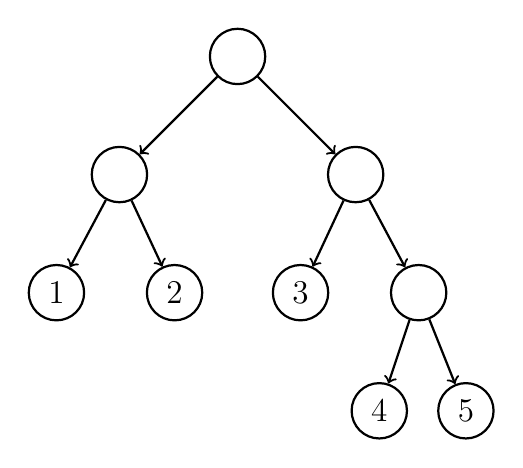
\begin{tikzpicture}
        [node/.style={circle,draw,minimum size=2em, thick, font=\large},
        nodeGray/.style={circle,draw,minimum size=2em, thick, font=\large, fill=gray!55}]
        \node[node] (D) at (0,0) {};
        \node[node] (B) at (-1.5,-1.5) {};
        \node[node] (A) at (-2.3,-3) {$1$};
        \node[node] (C) at (-0.8,-3) {$2$};
        \node[node] (E) at (0.8,-3) {$3$};
        \node[node] (F) at (1.5,-1.5) {};
        \node[node] (G) at (2.3,-3) {};
        \node[node] (H) at (1.8,-4.5) {$4$};
        \node[node] (I) at (2.9,-4.5) {$5$};
        
        \draw[thick, ->] (D) -- (B);%node[midway, left, yshift=0.15cm, xshift=0.08cm] {\textbf{E}};
        \draw[thick, ->] (B) -- (A);%node[midway, left, yshift=0.15cm, xshift=0.08cm] {\textbf{E}};
        \draw[thick, ->] (B) -- (C);%node[midway, right, yshift=0.15cm, xshift=-0.08cm] {\textbf{D}};
        \draw[thick, ->] (G) -- (I);%node[midway, right, yshift=0.15cm, xshift=-0.08cm] {\textbf{D}};
        \draw[thick, ->] (G) -- (H);%node[midway, left, yshift=0.15cm, xshift=0.08cm] {\textbf{E}};
        
        \draw[thick, ->] (D) -- (F);%node[midway, right, yshift=0.15cm, xshift=-0.08cm] {\textbf{D}};
        \draw[thick, ->] (F) -- (E);%node[midway, left, yshift=0.15cm, xshift=0.08cm] {\textbf{E}};
        \draw[thick, ->] (F) -- (G);%node[midway, right, yshift=0.15cm, xshift=-0.08cm] {\textbf{D}};
    
    \end{tikzpicture}
    \caption{Uma árvore de referência $\cT$ para o conjunto $P_X$ de pontos da sequência $X = (3,1,4,2,5)$ de acessos.}
\label{fig:arvore_de_referencia_exemplo_inicial}
\end{figure}

Sejam $\cT_{E}$ e $\cT_{D}$ respectivamente a subárvore esquerda e a subárvore direita da raiz de $\cT$, e sejam $P_E = \{p \in P \mid p.x \in \cT_E\}$ e $P_D = \{p \in P \mid p.x \in \cT_D\}$. Definimos $a(P,\cT) = \emph{intercala}(P_E.y, P_D.y)$, que mostra quanto se intercalam os pontos em $P_E$ e $P_D$ de maneira cronológica. Por fim, definimos a \textit{delimitação da alternância} para um conjunto $P$ de pontos em relação à árvore de referência $\cT$ como:

\begin{center}
\Alt$_\cT(P) = a(P,\cT) +$ \Alt$_{\cT_E}(P_E) + $ \Alt$_{\cT_D}(P_D)$.
\end{center}

Veja um exemplo na Figura~\ref{fig:exemplo_alternancia}.

Note que a delimitação da alternância de um conjunto de pontos pode ter valores diferentes dependendo da escolha da árvore de referência. Veja a Figura~\ref{fig:alternancia_diferente}. Assim, definimos a delimitação da alternância para uma sequência $X$ de acessos como o valor da maior delimitação da alternância para a visão geométrica de $X$ em relação a uma árvore de referência. Formalmente
\begin{center}
\Alt$(X) = \max_\cT$ \Alt$_\cT(P_X)$.
\end{center}
\begin{figure}
    \begin{minipage}[c]{0.3\textwidth} % Alinhar ao centro
        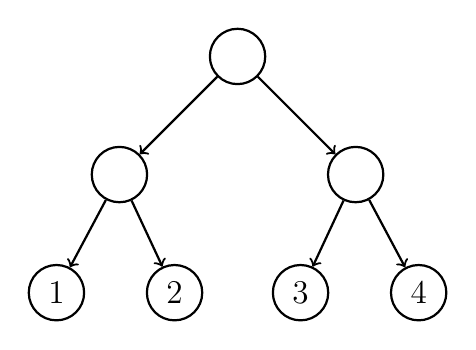
\begin{tikzpicture}
            [node/.style={circle,draw,minimum size=2em, thick, font=\large},
        nodeGray/.style={circle,draw,minimum size=2em, thick, font=\large, fill=gray!55}]
            \node[node] (D) at (0,0) {};
            \node[node] (B) at (-1.5,-1.5) {};
            \node[node] (A) at (-2.3,-3) {$1$};
            \node[node] (C) at (-0.8,-3) {$2$};
            \node[node] (E) at (0.8,-3) {$3$};
            \node[node] (F) at (1.5,-1.5) {};
            \node[node] (G) at (2.3,-3) {$4$};
            
            \draw[thick, ->] (D) -- (B); % node[midway, left, yshift=0.15cm, xshift=0.08cm] {\textbf{E}};
            \draw[thick, ->] (B) -- (A); % node[midway, left, yshift=0.15cm, xshift=0.08cm] {\textbf{E}};
            \draw[thick, ->] (B) -- (C); % node[midway, right, yshift=0.15cm, xshift=-0.08cm] {\textbf{D}};
            
            \draw[thick, ->] (D) -- (F); % node[midway, right, yshift=0.15cm, xshift=-0.08cm] {\textbf{D}};
            \draw[thick, ->] (F) -- (E); % node[midway, left, yshift=0.15cm, xshift=0.08cm] {\textbf{E}};
            \draw[thick, ->] (F) -- (G); % node[midway, right, yshift=0.15cm, xshift=-0.08cm] {\textbf{D}};
        \end{tikzpicture}
    \end{minipage} \hfill
    \begin{minipage}[c]{0.59\textwidth} % Alinhar ao centro
        \vfill % Preenche o espaço vertical
        \begin{tabular}{>{\centering\arraybackslash}p{1.4cm} >{\centering\arraybackslash}p{5cm} >{\centering\arraybackslash}p{1.5cm}} % Define as larguras das colunas
            \Alt & $mix(E,D)$ & $\emph{intercala}$ \\
            \hline
            $a(P,\cT)$ & \textbf{DEEDED}  & 5 \\
            \Alt$_{\cT_E}(P_E)$ & \textbf{DED}  & 3  \\
            \Alt$_{\cT_D}(P_D)$ & \textbf{EDE}  & 3  \\
            \hline
            \Alt$_\cT(P_X)$  &   & 11  \\
        \end{tabular}
        \vfill % Preenche o espaço vertical
    \end{minipage}
    \caption{Árvore de referência $\cT$ e \Alt$_\cT(P_X)$ para a sequência $X = (3,2,1,4,2,3)$ de acessos.}
\label{fig:exemplo_alternancia}
\end{figure}

\begin{figure}
    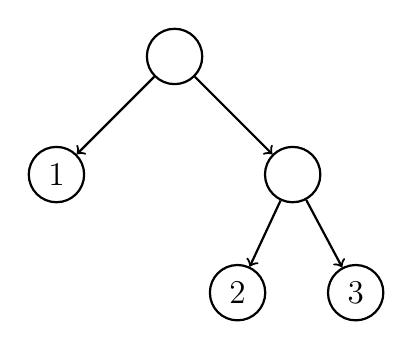
\begin{tikzpicture}
        [node/.style={circle,draw,minimum size=2em, thick, font=\large},
        nodeGray/.style={circle,draw,minimum size=2em, thick, font=\large, fill=gray!55}]
        \node[node] (D) at (0,0) {};
        \node[node] (B) at (-1.5,-1.5) {$1$};
        \node[node] (E) at (0.8,-3) {$2$};
        \node[node] (F) at (1.5,-1.5) {};
        \node[node] (G) at (2.3,-3) {$3$};
        
        \draw[thick, ->] (D) -- (B); % node[midway, left, yshift=0.15cm, xshift=0.08cm] {\textbf{E}};
        
        \draw[thick, ->] (D) -- (F); % node[midway, right, yshift=0.15cm, xshift=-0.08cm] {\textbf{D}};
        \draw[thick, ->] (F) -- (E); % node[midway, left, yshift=0.15cm, xshift=0.08cm] {\textbf{E}};
        \draw[thick, ->] (F) -- (G); % node[midway, right, yshift=0.15cm, xshift=-0.08cm] {\textbf{D}};
    \end{tikzpicture}
    \hspace{1cm}
    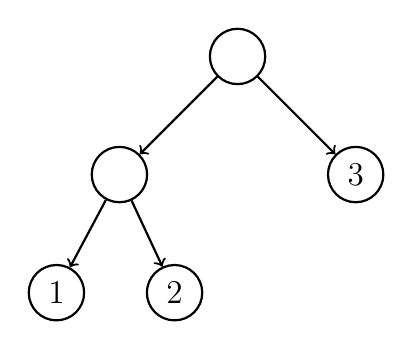
\begin{tikzpicture}
        [node/.style={circle,draw,minimum size=2em, thick, font=\large},
        nodeGray/.style={circle,draw,minimum size=2em, thick, font=\large, fill=gray!55}]
        \node[node] (D) at (0,0) {};
        \node[node] (B) at (-1.5,-1.5) {};
        \node[node] (A) at (-2.3,-3) {$1$};
        \node[node] (C) at (-0.8,-3) {$2$};
        \node[node] (F) at (1.5,-1.5) {$3$};
        
        \draw[thick, ->] (D) -- (B); % node[midway, left, yshift=0.15cm, xshift=0.08cm] {\textbf{E}};
        \draw[thick, ->] (B) -- (A); % node[midway, left, yshift=0.15cm, xshift=0.08cm] {\textbf{E}};
        \draw[thick, ->] (B) -- (C); % node[midway, right, yshift=0.15cm, xshift=-0.08cm] {\textbf{D}};
        
        \draw[thick, ->] (D) -- (F); % node[midway, right, yshift=0.15cm, xshift=-0.08cm] {\textbf{D}};
    \end{tikzpicture}
    \caption{À esquerda $\cT_1$ e à direita $\cT_2$. Para a sequência $X = (1,3,2)$ de acessos, \Alt$_{\cT_1}(P_X) = 4$, enquanto que \Alt$_{\cT_2}(P_X) = 5$.}
\label{fig:alternancia_diferente}
\end{figure}

%\Alt$_{\cT_E}(P_E)

Para contribuir com a intuição do leitor, a seguir mostraremos uma maneira alternativa e bem mais informal de entender essa delimitação. Podemos pensar nas árvores de referência como árvores binárias de busca com as chaves armazenadas nas folhas e assim é possível contabilizar essa delimitação simulando buscas pelos rótulos das folhas dessa árvore. Para todo nó não-folha de $\cT$, definimos como \textit{filho preferido} deste nó o filho mais recentemente visitado numa busca, podendo ser o filho esquerdo, o filho direito ou, se nenhum dos dois filhos tiver sido visitado ainda, o valor nulo.

Dada uma sequência $X$ de acessos, considere uma árvore de referência $\cT$ em relação a $P_X$. Simule o algoritmo tradicional de busca em ABB que não faz rotações para buscar os valores de $X$ em $\cT$. Veja a Figura~\ref{fig:alternancia_abordagem_informal}. Assim, \Alt$_\cT(X)$ é o somatório do número de vezes que o filho preferido de cada nó intermediário é alterado durante as buscas de $X$. Analogamente, \Alt$(X) = \max_\cT$ \Alt$_\cT(X)$. Então, \Alt$(X)$ é o somatório do número de vezes que o filho preferido de cada nó intermediário é alterado em uma árvore de referência que maximiza esse número.

Infelizmente essa delimitação não é justa se permitirmos repetições na sequência $X$. Uma maneira fácil de perceber que $\OPT(X)$ pode ser muito maior que \Alt$(X)$ é observando como a delimitação se comporta quando $X$ possui repetições do mesmo acesso consecutivamente. Quando simulamos a mesma busca consecutivas vezes em uma árvore de referência, nenhum filho preferido é alterado, então a delimitação não aumenta. Sabemos que todo acesso tem custo maior ou igual a 1 e assim $\OPT(X) \geq m$, mas devido a essas repetições, é possível que $m$ seja arbitrariamente maior que \Alt$(X)$. Para entender melhor o argumento acima, se atente às últimas duas simulações de busca na Figura~\ref{fig:alternancia_abordagem_informal}.

\begin{figure}
    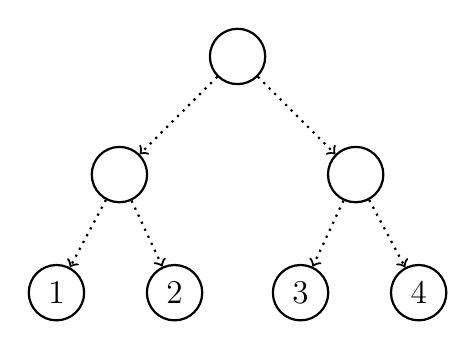
\begin{tikzpicture}
        [node/.style={circle,draw,minimum size=2em, thick, font=\large},
        nodeGray/.style={circle,draw,minimum size=2em, thick, font=\large, fill=gray!55}]
        \node[node] (D) at (0,0) {};
        \node[node] (B) at (-1.5,-1.5) {};
        \node[node] (A) at (-2.3,-3) {$1$};
        \node[node] (C) at (-0.8,-3) {$2$};
        \node[node] (E) at (0.8,-3) {$3$};
        \node[node] (F) at (1.5,-1.5) {};
        \node[node] (G) at (2.3,-3) {$4$};
        
        \draw[thick, dotted, ->] (D) -- (B);%node[midway, left, yshift=0.15cm, xshift=0.08cm] {\textbf{E}};
        \draw[thick, dotted, ->] (B) -- (A);%node[midway, left, yshift=0.15cm, xshift=0.08cm] {\textbf{E}};
        \draw[thick, dotted, ->] (B) -- (C);%node[midway, right, yshift=0.15cm, xshift=-0.08cm] {\textbf{D}};
        
        \draw[thick, dotted, ->] (D) -- (F);%node[midway, right, yshift=0.15cm, xshift=-0.08cm] {\textbf{D}};
        \draw[thick, dotted, ->] (F) -- (E);%node[midway, left, yshift=0.15cm, xshift=0.08cm] {\textbf{E}};
        \draw[thick, dotted, ->] (F) -- (G);%node[midway, right, yshift=0.15cm, xshift=-0.08cm] {\textbf{D}};
    
    \end{tikzpicture}
    \hspace{1cm}
    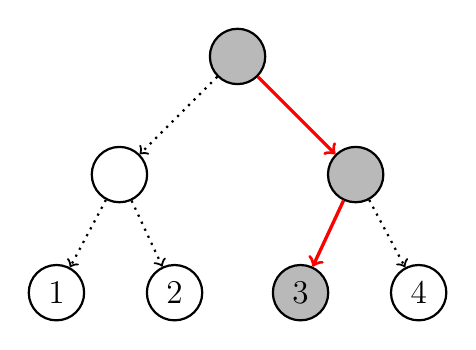
\begin{tikzpicture}
        [node/.style={circle,draw,minimum size=2em, thick, font=\large},
        nodeGray/.style={circle,draw,minimum size=2em, thick, font=\large, fill=gray!55}]
        \node[nodeGray] (D) at (0,0) {};
        \node[node] (B) at (-1.5,-1.5) {};
        \node[node] (A) at (-2.3,-3) {$1$};
        \node[node] (C) at (-0.8,-3) {$2$};
        \node[nodeGray] (E) at (0.8,-3) {$3$};
        \node[nodeGray] (F) at (1.5,-1.5) {};
        \node[node] (G) at (2.3,-3) {$4$};
        
        \draw[thick, dotted, ->] (D) -- (B);%node[midway, left, yshift=0.15cm, xshift=0.08cm] {\textbf{E}};
        \draw[thick, dotted, ->] (B) -- (A);%node[midway, left, yshift=0.15cm, xshift=0.08cm] {\textbf{E}};
        \draw[thick, dotted, ->] (B) -- (C);%node[midway, right, yshift=0.15cm, xshift=-0.08cm] {\textbf{D}};
        
        \draw[very thick, ->, red] (D) -- (F);%node[midway, right, yshift=0.15cm, xshift=-0.08cm] {\textbf{D}};
        \draw[very thick, ->, red] (F) -- (E);%node[midway, left, yshift=0.15cm, xshift=0.08cm] {\textbf{E}};
        \draw[thick, dotted, ->] (F) -- (G);%node[midway, right, yshift=0.15cm, xshift=-0.08cm] {\textbf{D}};
    
    \end{tikzpicture}
    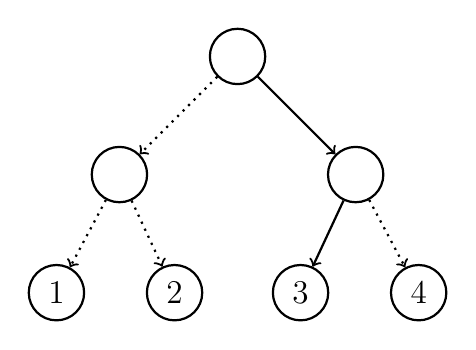
\begin{tikzpicture}
        [node/.style={circle,draw,minimum size=2em, thick, font=\large},
        nodeGray/.style={circle,draw,minimum size=2em, thick, font=\large, fill=gray!55}]
        \node[node] (D) at (0,0) {};
        \node[node] (B) at (-1.5,-1.5) {};
        \node[node] (A) at (-2.3,-3) {$1$};
        \node[node] (C) at (-0.8,-3) {$2$};
        \node[node] (E) at (0.8,-3) {$3$};
        \node[node] (F) at (1.5,-1.5) {};
        \node[node] (G) at (2.3,-3) {$4$};
        
        \draw[thick, dotted, ->] (D) -- (B);%node[midway, left, yshift=0.15cm, xshift=0.08cm] {\textbf{E}};
        \draw[thick, dotted, ->] (B) -- (A);%node[midway, left, yshift=0.15cm, xshift=0.08cm] {\textbf{E}};
        \draw[thick, dotted, ->] (B) -- (C);%node[midway, right, yshift=0.15cm, xshift=-0.08cm] {\textbf{D}};
        
        \draw[thick, ->] (D) -- (F);%node[midway, right, yshift=0.15cm, xshift=-0.08cm] {\textbf{D}};
        \draw[thick, ->] (F) -- (E);%node[midway, left, yshift=0.15cm, xshift=0.08cm] {\textbf{E}};
        \draw[thick, dotted, ->] (F) -- (G);%node[midway, right, yshift=0.15cm, xshift=-0.08cm] {\textbf{D}};
    
    \end{tikzpicture}
    \hspace{1cm}
    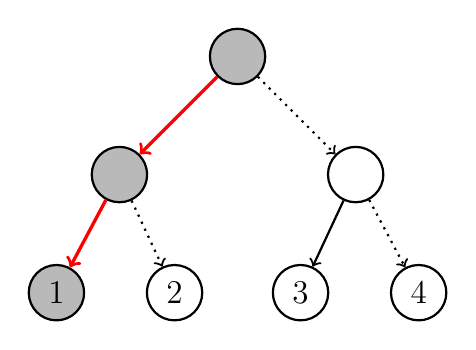
\begin{tikzpicture}
        [node/.style={circle,draw,minimum size=2em, thick, font=\large},
        nodeGray/.style={circle,draw,minimum size=2em, thick, font=\large, fill=gray!55}]
        \node[nodeGray] (D) at (0,0) {};
        \node[nodeGray] (B) at (-1.5,-1.5) {};
        \node[nodeGray] (A) at (-2.3,-3) {$1$};
        \node[node] (C) at (-0.8,-3) {$2$};
        \node[node] (E) at (0.8,-3) {$3$};
        \node[node] (F) at (1.5,-1.5) {};
        \node[node] (G) at (2.3,-3) {$4$};
        
        \draw[very thick, ->, red] (D) -- (B);%node[midway, left, yshift=0.15cm, xshift=0.08cm] {\textbf{E}};
        \draw[very thick, ->, red] (B) -- (A);%node[midway, left, yshift=0.15cm, xshift=0.08cm] {\textbf{E}};
        \draw[thick, dotted, ->] (B) -- (C);%node[midway, right, yshift=0.15cm, xshift=-0.08cm] {\textbf{D}};
        
        \draw[thick, dotted, ->] (D) -- (F);%node[midway, right, yshift=0.15cm, xshift=-0.08cm] {\textbf{D}};
        \draw[thick, ->] (F) -- (E);%node[midway, left, yshift=0.15cm, xshift=0.08cm] {\textbf{E}};
        \draw[thick, dotted, ->] (F) -- (G);%node[midway, right, yshift=0.15cm, xshift=-0.08cm] {\textbf{D}};
    
    \end{tikzpicture}
    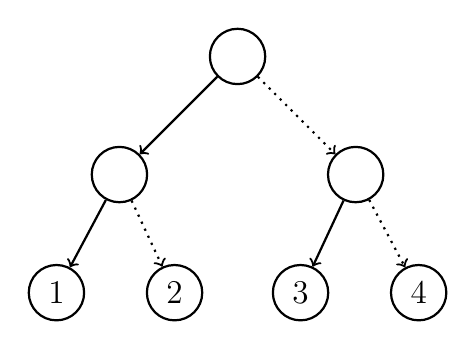
\begin{tikzpicture}
        [node/.style={circle,draw,minimum size=2em, thick, font=\large},
        nodeGray/.style={circle,draw,minimum size=2em, thick, font=\large, fill=gray!55}]
        \node[node] (D) at (0,0) {};
        \node[node] (B) at (-1.5,-1.5) {};
        \node[node] (A) at (-2.3,-3) {$1$};
        \node[node] (C) at (-0.8,-3) {$2$};
        \node[node] (E) at (0.8,-3) {$3$};
        \node[node] (F) at (1.5,-1.5) {};
        \node[node] (G) at (2.3,-3) {$4$};
        
        \draw[thick, ->] (D) -- (B);%node[midway, left, yshift=0.15cm, xshift=0.08cm] {\textbf{E}};
        \draw[thick, ->] (B) -- (A);%node[midway, left, yshift=0.15cm, xshift=0.08cm] {\textbf{E}};
        \draw[thick, dotted, ->] (B) -- (C);%node[midway, right, yshift=0.15cm, xshift=-0.08cm] {\textbf{D}};
        
        \draw[thick, dotted, ->] (D) -- (F);%node[midway, right, yshift=0.15cm, xshift=-0.08cm] {\textbf{D}};
        \draw[thick, ->] (F) -- (E);%node[midway, left, yshift=0.15cm, xshift=0.08cm] {\textbf{E}};
        \draw[thick, dotted, ->] (F) -- (G);%node[midway, right, yshift=0.15cm, xshift=-0.08cm] {\textbf{D}};
    
    \end{tikzpicture}
    \hspace{1cm}
    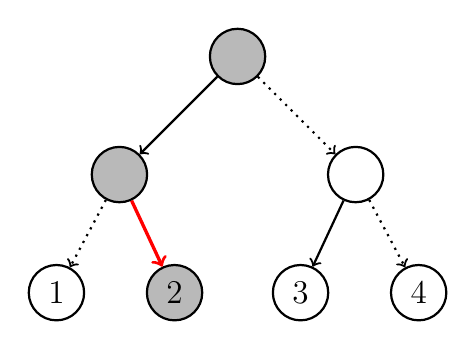
\begin{tikzpicture}
        [node/.style={circle,draw,minimum size=2em, thick, font=\large},
        nodeGray/.style={circle,draw,minimum size=2em, thick, font=\large, fill=gray!55}]
        \node[nodeGray] (D) at (0,0) {};
        \node[nodeGray] (B) at (-1.5,-1.5) {};
        \node[node] (A) at (-2.3,-3) {$1$};
        \node[nodeGray] (C) at (-0.8,-3) {$2$};
        \node[node] (E) at (0.8,-3) {$3$};
        \node[node] (F) at (1.5,-1.5) {};
        \node[node] (G) at (2.3,-3) {$4$};
        
        \draw[thick, ->] (D) -- (B);%node[midway, left, yshift=0.15cm, xshift=0.08cm] {\textbf{E}};
        \draw[thick, dotted, ->] (B) -- (A);%node[midway, left, yshift=0.15cm, xshift=0.08cm] {\textbf{E}};
        \draw[very thick, ->, red] (B) -- (C);%node[midway, right, yshift=0.15cm, xshift=-0.08cm] {\textbf{D}};
        
        \draw[thick, dotted, ->] (D) -- (F);%node[midway, right, yshift=0.15cm, xshift=-0.08cm] {\textbf{D}};
        \draw[thick, ->] (F) -- (E);%node[midway, left, yshift=0.15cm, xshift=0.08cm] {\textbf{E}};
        \draw[thick, dotted, ->] (F) -- (G);%node[midway, right, yshift=0.15cm, xshift=-0.08cm] {\textbf{D}};
    
    \end{tikzpicture}
    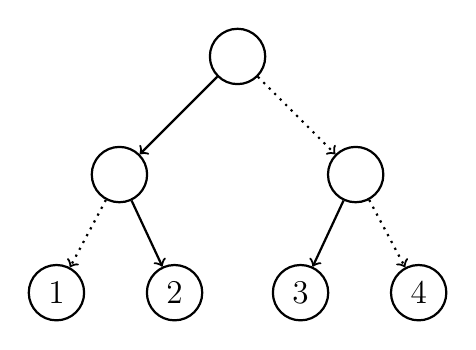
\begin{tikzpicture}
        [node/.style={circle,draw,minimum size=2em, thick, font=\large},
        nodeGray/.style={circle,draw,minimum size=2em, thick, font=\large, fill=gray!55}]
        \node[node] (D) at (0,0) {};
        \node[node] (B) at (-1.5,-1.5) {};
        \node[node] (A) at (-2.3,-3) {$1$};
        \node[node] (C) at (-0.8,-3) {$2$};
        \node[node] (E) at (0.8,-3) {$3$};
        \node[node] (F) at (1.5,-1.5) {};
        \node[node] (G) at (2.3,-3) {$4$};
        
        \draw[thick, ->] (D) -- (B);%node[midway, left, yshift=0.15cm, xshift=0.08cm] {\textbf{E}};
        \draw[thick, dotted, ->] (B) -- (A);%node[midway, left, yshift=0.15cm, xshift=0.08cm] {\textbf{E}};
        \draw[thick, ->] (B) -- (C);%node[midway, right, yshift=0.15cm, xshift=-0.08cm] {\textbf{D}};
        
        \draw[thick, dotted, ->] (D) -- (F);%node[midway, right, yshift=0.15cm, xshift=-0.08cm] {\textbf{D}};
        \draw[thick, ->] (F) -- (E);%node[midway, left, yshift=0.15cm, xshift=0.08cm] {\textbf{E}};
        \draw[thick, dotted, ->] (F) -- (G);%node[midway, right, yshift=0.15cm, xshift=-0.08cm] {\textbf{D}};
    
    \end{tikzpicture}
    \hspace{1cm}
    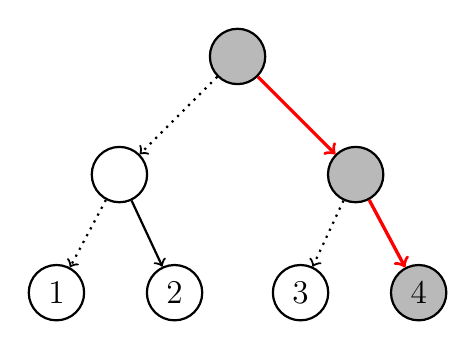
\begin{tikzpicture}
        [node/.style={circle,draw,minimum size=2em, thick, font=\large},
        nodeGray/.style={circle,draw,minimum size=2em, thick, font=\large, fill=gray!55}]
        \node[nodeGray] (D) at (0,0) {};
        \node[node] (B) at (-1.5,-1.5) {};
        \node[node] (A) at (-2.3,-3) {$1$};
        \node[node] (C) at (-0.8,-3) {$2$};
        \node[node] (E) at (0.8,-3) {$3$};
        \node[nodeGray] (F) at (1.5,-1.5) {};
        \node[nodeGray] (G) at (2.3,-3) {$4$};
        
        \draw[thick, dotted, ->] (D) -- (B);%node[midway, left, yshift=0.15cm, xshift=0.08cm] {\textbf{E}};
        \draw[thick, dotted, ->] (B) -- (A);%node[midway, left, yshift=0.15cm, xshift=0.08cm] {\textbf{E}};
        \draw[thick, ->] (B) -- (C);%node[midway, right, yshift=0.15cm, xshift=-0.08cm] {\textbf{D}};
        
        \draw[very thick, ->, red] (D) -- (F);%node[midway, right, yshift=0.15cm, xshift=-0.08cm] {\textbf{D}};
        \draw[thick, dotted, ->] (F) -- (E);%node[midway, left, yshift=0.15cm, xshift=0.08cm] {\textbf{E}};
        \draw[very thick, ->, red] (F) -- (G);%node[midway, right, yshift=0.15cm, xshift=-0.08cm] {\textbf{D}};
    \end{tikzpicture}
    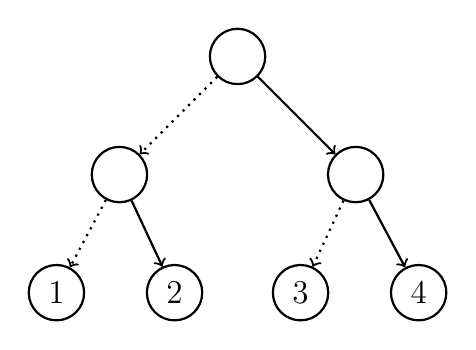
\begin{tikzpicture}
        [node/.style={circle,draw,minimum size=2em, thick, font=\large},
        nodeGray/.style={circle,draw,minimum size=2em, thick, font=\large, fill=gray!55}]
        \node[node] (D) at (0,0) {};
        \node[node] (B) at (-1.5,-1.5) {};
        \node[node] (A) at (-2.3,-3) {$1$};
        \node[node] (C) at (-0.8,-3) {$2$};
        \node[node] (E) at (0.8,-3) {$3$};
        \node[node] (F) at (1.5,-1.5) {};
        \node[node] (G) at (2.3,-3) {$4$};
        
        \draw[thick, dotted, ->] (D) -- (B);%node[midway, left, yshift=0.15cm, xshift=0.08cm] {\textbf{E}};
        \draw[thick, dotted, ->] (B) -- (A);%node[midway, left, yshift=0.15cm, xshift=0.08cm] {\textbf{E}};
        \draw[thick, ->] (B) -- (C);%node[midway, right, yshift=0.15cm, xshift=-0.08cm] {\textbf{D}};
        
        \draw[thick, ->] (D) -- (F);%node[midway, right, yshift=0.15cm, xshift=-0.08cm] {\textbf{D}};
        \draw[thick, dotted, ->] (F) -- (E);%node[midway, left, yshift=0.15cm, xshift=0.08cm] {\textbf{E}};
        \draw[thick, ->] (F) -- (G);%node[midway, right, yshift=0.15cm, xshift=-0.08cm] {\textbf{D}};
    \end{tikzpicture}
    \hspace{1cm}
    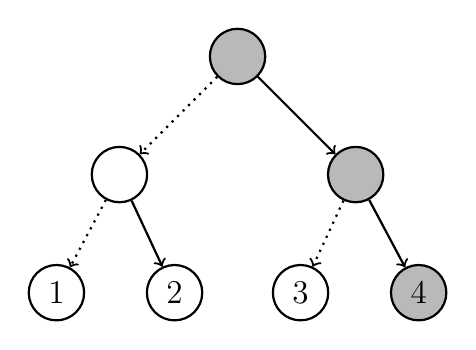
\begin{tikzpicture}
        [node/.style={circle,draw,minimum size=2em, thick, font=\large},
        nodeGray/.style={circle,draw,minimum size=2em, thick, font=\large, fill=gray!55}]
        \node[nodeGray] (D) at (0,0) {};
        \node[node] (B) at (-1.5,-1.5) {};
        \node[node] (A) at (-2.3,-3) {$1$};
        \node[node] (C) at (-0.8,-3) {$2$};
        \node[node] (E) at (0.8,-3) {$3$};
        \node[nodeGray] (F) at (1.5,-1.5) {};
        \node[nodeGray] (G) at (2.3,-3) {$4$};
        
        \draw[thick, dotted, ->] (D) -- (B);%node[midway, left, yshift=0.15cm, xshift=0.08cm] {\textbf{E}};
        \draw[thick, dotted, ->] (B) -- (A);%node[midway, left, yshift=0.15cm, xshift=0.08cm] {\textbf{E}};
        \draw[thick, ->] (B) -- (C);%node[midway, right, yshift=0.15cm, xshift=-0.08cm] {\textbf{D}};
        
        \draw[thick, ->] (D) -- (F);%node[midway, right, yshift=0.15cm, xshift=-0.08cm] {\textbf{D}};
        \draw[thick, dotted, ->] (F) -- (E);%node[midway, left, yshift=0.15cm, xshift=0.08cm] {\textbf{E}};
        \draw[thick, ->] (F) -- (G);%node[midway, right, yshift=0.15cm, xshift=-0.08cm] {\textbf{D}};
    \end{tikzpicture}
    
    \caption{Cálculo de \Alt$_\cT(X)$ para a sequência $X = (3,1,2,4,4)$ de acessos e a árvore de referência $\cT$ ilustrada. À esquerda, as árvores antes da simulação de buscas. À direita, a simulação de cada busca. Os ponteiros que representam filhos preferidos estão por inteiro, enquanto que os ponteiros que representam filhos não-preferidos estão pontilhados. Durante as simulações de busca, estão em vermelho os filhos preferidos que foram alterados durante aquela busca. Note que \Alt$_\cT(X) = 7$, pois esse é o número de filhos preferidos alterados (ponteiros vermelhos) durante as buscas de $X$.}
\label{fig:alternancia_abordagem_informal}
\end{figure}

\section{Conjunto independente de retângulos a partir da alternância} \label{sec:alt_com_ret}

Nessa seção, mostraremos um algoritmo que encontra um conjunto independente de retângulos para $P_X$ a partir de uma sequência $X$ de acessos e uma árvore de referência. Lembre-se que $n$ denota o número de chaves consideradas e que a árvore de referência tem então $n$ folhas. Mostraremos que o conjunto de retângulos produzido pelo algoritmo tem pelo menos \Alt$(P_X) - (n - 1)$ retângulos. Na prática, o algoritmo encontrará pares de pontos de $P_X$ que representam retângulos.

Para facilitar o entendimento do leitor, aconselhamos acompanhar a descrição do algoritmo utilizando a Figura~\ref{fig:alternancia-retangulos}.
Considere a visão geométrica $P_X$ de uma sequência $X$ de acessos em um plano 2D e uma árvore de referência $\cT$ em relação a $P_X$ com $n$ folhas. Denotemos por $I$ o conjunto de pares de pontos que o algoritmo retornará ao fim da execução. Para um nó $x$ de $\cT$, seja $u$ o maior rótulo de um nó na subárvore esquerda de $x$ e $v$ o menor rótulo de um nó na subárvore direita de $x$. O algoritmo inicializa $I$ como o conjunto vazio e verifica o nó $r$, raiz de $\cT$, da seguinte forma: considere a reta vertical $\ell(r)$ no plano 2D com $x$-coordenada igual a $\frac{u+v}{2}$, adicione a $I$ todos os pares $(a,b)$ de pontos de $P_X$ consecutivos, onde $a$ está à esquerda de $\ell(r)$ e $b$ está à direita de $\ell(r)$. Em seguida, o algoritmo analisa recursivamente o filho esquerdo de $r$ em $\cT$ porém considerando apenas os pontos de $P_X$ à esquerda de $\ell(r)$ e analisa o filho direito de $r$ em $\cT$ porém considerando apenas os pontos de $P_X$ à direita de $\ell(r)$.

Claramente o conjunto de pares de pontos incluídos em $I$ ao processar um dos nós da árvore representa uma coleção independente de retângulos. Mostraremos que, para dois nós $w$ e $z$ de $\cT$, o conjunto de pares de pontos encontrado durante a análise do algoritmo para o nó $w$ representa retângulos independentes dos representados pelo conjunto de pares de pontos encontrado durante a análise do algoritmo para o nó $z$. Suponha que $w$ e $z$ não são descendentes um do outro em $\cT$. Então o subconjunto de $P_X$ considerado durante a análise do algoritmo para um desses nós está totalmente à esquerda do subconjunto do outro, logo os retângulos representados pelos pares de pontos de $w$ são diferentes e independentes dos retângulos de $z$. Suponha agora que $w$ é descendente de $z$. Então durante a análise do algoritmo para o nó $z$ são encontrados pares de pontos, onde um está à esquerda de $\ell(z)$ e outro está à direita. Porém, por $w$ ser descendente de $z$, o subconjunto de $P_X$ considerado durante a análise de $w$ possui apenas pontos de um lado da reta $\ell(z)$. Logo os conjuntos de pares de pontos encontrados pelo algoritmo para esses nós são disjuntos. Mais do que isso, se um retângulo de $w$ não for independente de um retângulo de $z$, então o par que representa um desses retângulos não era consecutivo quando esse foi incluído em $I$. Como os conjuntos de pares de pontos encontrados pelo algoritmo para dois nós diferentes são disjuntos, então o tamanho do conjunto $I$ ao final da execução do algoritmo é igual a somatória do número de pares de pontos adicionados a $I$ para cada um dos nós de $\cT$.

Perceba que todo par $(a,b)$ de pontos encontrado pelo algoritmo durante a análise do nó $w$ de $\cT$ representa uma alteração do filho preferido de $w$, uma vez que $a$ e $b$ estão em lados opostos da reta $\ell(w)$ e são consecutivos dentro do subconjunto de $P_X$ considerado. Nota-se que a alteração de filho preferido de valor nulo para outro valor é representada pelo ponto com menor $y$-coordenada dentro do subconjunto de $P_X$ considerado, ou seja, esta alteração não é representada por nenhum retângulo de $I$. Assim, nota-se que o tamanho de $I$ ao final da execução do algoritmo é, no mínimo, \Alt$(P_X) - (n - 1)$, pois há $n - 1$ nós intermediários em $\cT$. Se considerarmos $\Alt(P_X) = \Omega(n)$, então o algoritmo encontra $\Oh(\Alt(P_X))$ retângulos e esse desconto de $n - 1$ é assintoticamente absorvido pelo termo $\Omega(n)$.


\begin{figure}
    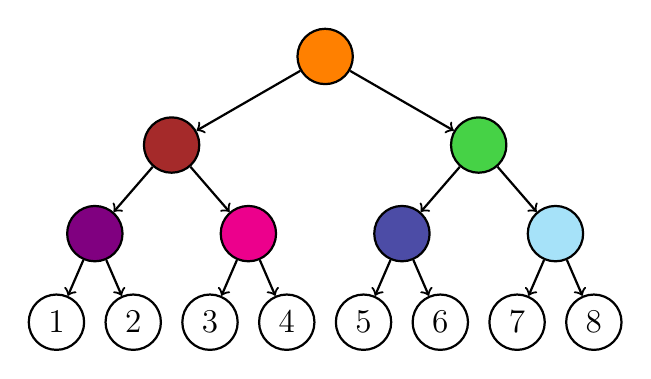
\begin{tikzpicture}[scale=0.75,
        node/.style={circle,draw,minimum size=2em, thick, font=\large},
        nodeGray/.style={circle,draw,minimum size=2em, thick, font=\large, fill=gray!55}]
        
        \node[node, fill=orange] (H) at (0,0) {};
        \node[node, fill=Brown] (D) at (-2.6,-1.5) {};
        \node[node, fill=Purple] (B) at (-3.9,-3) {};
        \node[node] (A) at (-4.55,-4.5) {$1$};
        \node[node] (C) at (-3.25,-4.5) {$2$};
        \node[node, fill=magenta] (F) at (-1.3,-3) {};
        \node[node] (E) at (-1.95,-4.5) {$3$};
        \node[node] (G) at (-0.65,-4.5) {$4$};


        \node[node, fill=LimeGreen!90] (L) at (2.6,-1.5) {};
        \node[node, fill=cyan!35] (J) at (3.9,-3) {};
        \node[node] (I) at (4.55,-4.5) {$8$};
        \node[node] (K) at (3.25,-4.5) {$7$};
        \node[node, fill=NavyBlue!70] (N) at (1.3,-3) {};
        \node[node] (M) at (1.95,-4.5) {$6$};
        \node[node] (O) at (0.65,-4.5) {$5$};
        
        \draw[thick, ->] (H) -- (D);
        \draw[thick, ->] (H) -- (L);
        \draw[thick, ->] (D) -- (B);
        \draw[thick, ->] (D) -- (F);
        \draw[thick, ->] (B) -- (A);
        \draw[thick, ->] (B) -- (C);
        \draw[thick, ->] (F) -- (E);
        \draw[thick, ->] (F) -- (G);

        \draw[thick, ->] (L) -- (J);
        \draw[thick, ->] (L) -- (N);
        \draw[thick, ->] (J) -- (I);
        \draw[thick, ->] (J) -- (K);
        \draw[thick, ->] (N) -- (M);
        \draw[thick, ->] (N) -- (O);
    
    \end{tikzpicture}
    \\
    \vspace{0.3cm}
    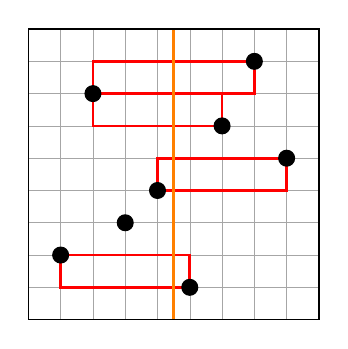
\begin{tikzpicture}[scale=0.41]
        \draw[very thin, gray!70] (0,0) grid (9,9);

        \draw[red, line width=1pt] (5,1) rectangle (1,2);
        \draw[red, line width=1pt] (4,4) rectangle (8,5);
        \draw[red, line width=1pt] (6,6) rectangle (2,7);
        \draw[red, line width=1pt] (7,8) rectangle (2,7);

        \draw[orange, line width=1pt] (4.5,0) -- (4.5,9);
        
        \filldraw[black] (5,1) circle (7pt);
        \filldraw[black] (1,2) circle (7pt);
        \filldraw[black] (3,3) circle (7pt);
        \filldraw[black] (4,4) circle (7pt);
        \filldraw[black] (8,5) circle (7pt);
        \filldraw[black] (6,6) circle (7pt);
        \filldraw[black] (2,7) circle (7pt);
        \filldraw[black] (7,8) circle (7pt);
        \draw[black, line width=0.5pt] (0,0) rectangle (9,9);
    \end{tikzpicture}
    \\
    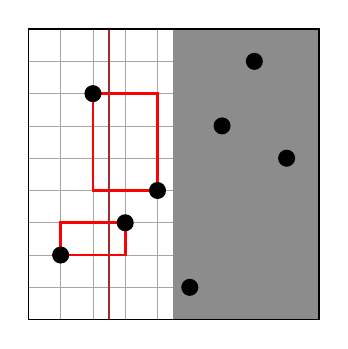
\begin{tikzpicture}[scale=0.41]
        \draw[very thin, gray!70] (0,0) grid (9,9);
        \draw[fill=gray!90, gray!90] (9,9) rectangle (4.5,0);

        \draw[red, line width=1pt] (1,2) rectangle (3,3);
        \draw[red, line width=1pt] (4,4) rectangle (2,7);

        \draw[Brown, line width=1pt] (2.5,0) -- (2.5,9);
        
        \filldraw[black] (5,1) circle (7pt);
        \filldraw[black] (1,2) circle (7pt);
        \filldraw[black] (3,3) circle (7pt);
        \filldraw[black] (4,4) circle (7pt);
        \filldraw[black] (8,5) circle (7pt);
        \filldraw[black] (6,6) circle (7pt);
        \filldraw[black] (2,7) circle (7pt);
        \filldraw[black] (7,8) circle (7pt);
        \draw[black, line width=0.5pt] (0,0) rectangle (9,9);
    \end{tikzpicture}
    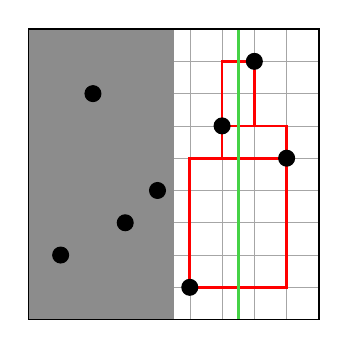
\begin{tikzpicture}[scale=0.41]
        \draw[very thin, gray!70] (0,0) grid (9,9);
        \draw[fill=gray!90, gray!90] (0,9) rectangle (4.5,0);

        \draw[red, line width=1pt] (5,1) rectangle (8,5);
        \draw[red, line width=1pt] (6,6) rectangle (8,5);
        \draw[red, line width=1pt] (6,6) rectangle (7,8);

        \draw[LimeGreen!90, line width=1pt] (6.5,0) -- (6.5,9);
        
        \filldraw[black] (5,1) circle (7pt);
        \filldraw[black] (1,2) circle (7pt);
        \filldraw[black] (3,3) circle (7pt);
        \filldraw[black] (4,4) circle (7pt);
        \filldraw[black] (8,5) circle (7pt);
        \filldraw[black] (6,6) circle (7pt);
        \filldraw[black] (2,7) circle (7pt);
        \filldraw[black] (7,8) circle (7pt);
        \draw[black, line width=0.5pt] (0,0) rectangle (9,9);
    \end{tikzpicture}
    \\
    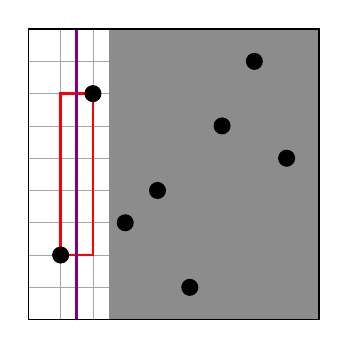
\begin{tikzpicture}[scale=0.41]
        \draw[very thin, gray!70] (0,0) grid (9,9);
        \draw[fill=gray!90, gray!90] (9,9) rectangle (2.5,0);

        \draw[red, line width=1pt] (1,2) rectangle (2,7);

        \draw[Purple, line width=1pt] (1.5,0) -- (1.5,9);
        
        \filldraw[black] (5,1) circle (7pt);
        \filldraw[black] (1,2) circle (7pt);
        \filldraw[black] (3,3) circle (7pt);
        \filldraw[black] (4,4) circle (7pt);
        \filldraw[black] (8,5) circle (7pt);
        \filldraw[black] (6,6) circle (7pt);
        \filldraw[black] (2,7) circle (7pt);
        \filldraw[black] (7,8) circle (7pt);
        \draw[black, line width=0.5pt] (0,0) rectangle (9,9);
    \end{tikzpicture}
    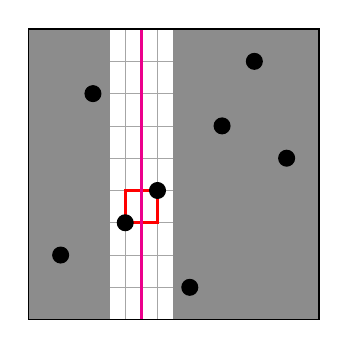
\begin{tikzpicture}[scale=0.41]
        \draw[very thin, gray!70] (0,0) grid (9,9);
        \draw[fill=gray!90, gray!90] (9,9) rectangle (4.5,0);
        \draw[fill=gray!90, gray!90] (0,9) rectangle (2.5,0);

        \draw[red, line width=1pt] (3,3) rectangle (4,4);

        \draw[magenta, line width=1pt] (3.5,0) -- (3.5,9);
        
        \filldraw[black] (5,1) circle (7pt);
        \filldraw[black] (1,2) circle (7pt);
        \filldraw[black] (3,3) circle (7pt);
        \filldraw[black] (4,4) circle (7pt);
        \filldraw[black] (8,5) circle (7pt);
        \filldraw[black] (6,6) circle (7pt);
        \filldraw[black] (2,7) circle (7pt);
        \filldraw[black] (7,8) circle (7pt);
        \draw[black, line width=0.5pt] (0,0) rectangle (9,9);
    \end{tikzpicture}
    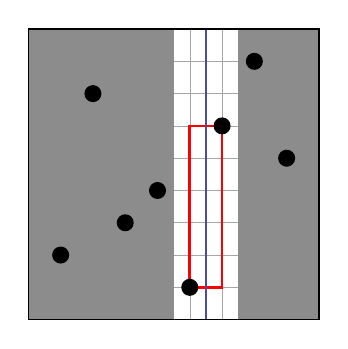
\begin{tikzpicture}[scale=0.41]
        \draw[very thin, gray!70] (0,0) grid (9,9);
        \draw[fill=gray!90, gray!90] (9,9) rectangle (6.5,0);
        \draw[fill=gray!90, gray!90] (0,9) rectangle (4.5,0);

        \draw[red, line width=1pt] (5,1) rectangle (6,6);

        \draw[NavyBlue!70, line width=1pt] (5.5,0) -- (5.5,9);
        
        \filldraw[black] (5,1) circle (7pt);
        \filldraw[black] (1,2) circle (7pt);
        \filldraw[black] (3,3) circle (7pt);
        \filldraw[black] (4,4) circle (7pt);
        \filldraw[black] (8,5) circle (7pt);
        \filldraw[black] (6,6) circle (7pt);
        \filldraw[black] (2,7) circle (7pt);
        \filldraw[black] (7,8) circle (7pt);
        \draw[black, line width=0.5pt] (0,0) rectangle (9,9);
    \end{tikzpicture}
    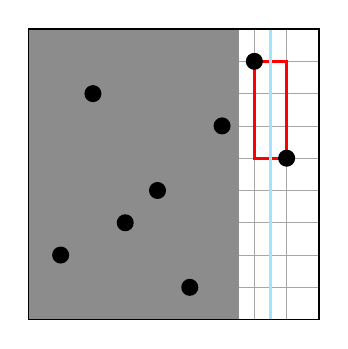
\begin{tikzpicture}[scale=0.41]
        \draw[very thin, gray!70] (0,0) grid (9,9);
        \draw[fill=gray!90, gray!90] (0,9) rectangle (6.5,0);
        \draw[red, line width=1pt] (8,5) rectangle (7,8);
        
        \draw[cyan!35, line width=1pt] (7.5,0) -- (7.5,9);
        
        \filldraw[black] (5,1) circle (7pt);
        \filldraw[black] (1,2) circle (7pt);
        \filldraw[black] (3,3) circle (7pt);
        \filldraw[black] (4,4) circle (7pt);
        \filldraw[black] (8,5) circle (7pt);
        \filldraw[black] (6,6) circle (7pt);
        \filldraw[black] (2,7) circle (7pt);
        \filldraw[black] (7,8) circle (7pt);
        \draw[black, line width=0.5pt] (0,0) rectangle (9,9);
    \end{tikzpicture}
    \caption{Em cima, uma árvore de referência em relação à visão geométrica da sequência de acessos $X = (5,1,3,4,8,6,2,7)$. Cada nó intermediário possui uma cor diferente. Abaixo, está ilustrada a execução do algoritmo recursivo que encontra um conjunto independente de $\Alt_\protect\cT(P_X) - (n - 1)$ retângulos. Cada linha vertical possui a cor do nó intermediário correspondente.}
\label{fig:alternancia-retangulos}
\end{figure}

\section{Delimitação do funil} \label{seção:funil}

Seja $P$ um conjunto de pontos. Definimos o \textit{lado esquerdo do funil} de um ponto $p$ de $P$ como o conjunto de pontos de $P$ que possuem as seguintes propriedades: estão à esquerda de $p$, abaixo de $p$ e o retângulo ortogonal que possui $p$ e algum ponto do lado esquerdo do funil de $p$ como vértices não possui nenhum outro ponto de $P$. Formalmente, 

{\centering $F_E(P,p) = \{q \in P \mid q.y < p.y \; e \; q.x < p.x \; e \; \{p,q\}\text{-retângulo é arboreamente insatisfeito}\}.$}

De maneira simétrica definimos o \textit{lado direito do funil} de $p$,

{\centering $F_D(P,p) = \{q \in P \mid q.y > p.y \; e \; q.x < p.x \; e \; \{p,q\}\text{-retângulo é arboreamente insatisfeito}\}.$}

Por fim, definimos o \textit{funil} de $p$ como a união do lado esquerdo do funil e do lado direito do funil de $p$, ou seja, $F_E(P,p) \cup F_D(P,p)$. Veja a Figura~\ref{fig:funil-apresentacao}.

É importante notar que cronologicamente os pontos do lado esquerdo do funil de qualquer ponto $p$ possuem $x$-coordenadas decrescentes. De maneira análoga, cronologicamente os pontos do lado direito do funil de qualquer ponto $p$ possuem $x$-coordenadas crescentes. Isso acontece por conta da propriedade de insatisfação arbórea do ponto $p$ com os pontos de seu funil.

\begin{comment}
    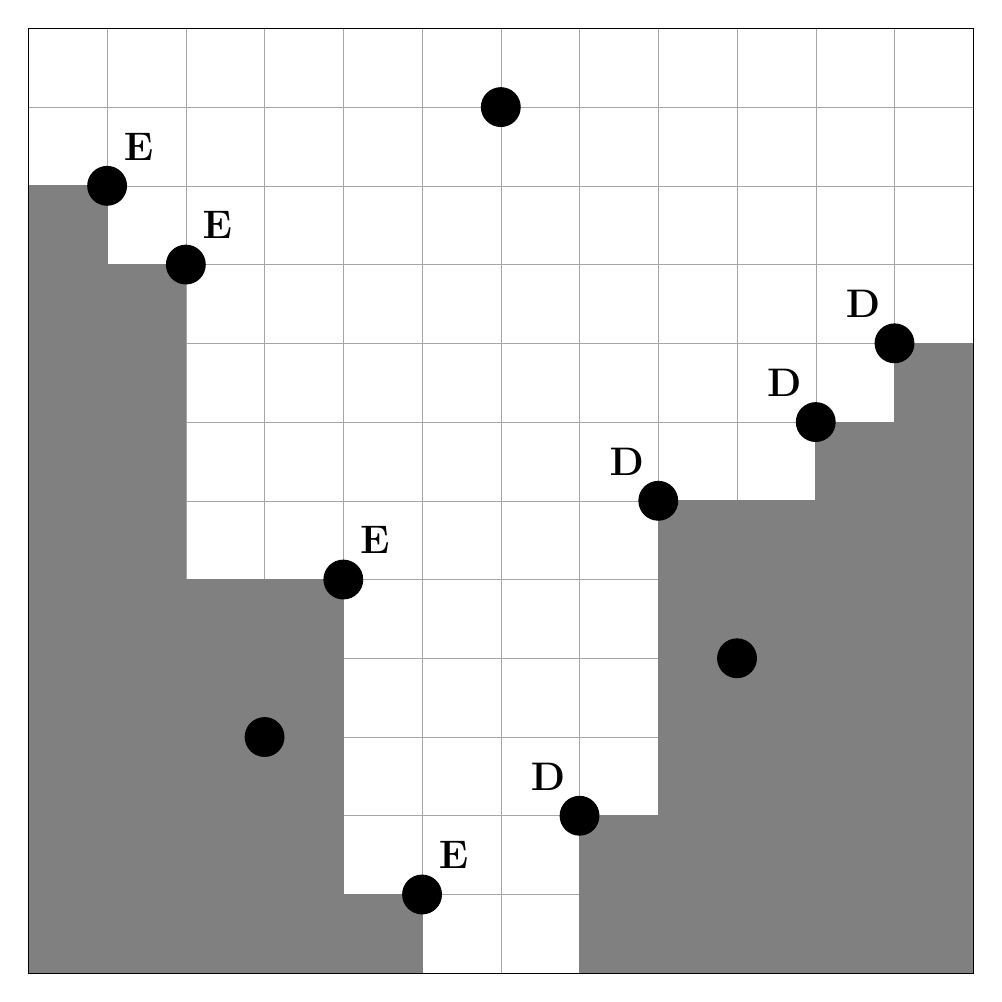
\begin{tikzpicture}[scale=1]
        \draw[very thin, gray!70] (0,0) grid (12,12);
        
        \draw[fill=gray, gray] (0,0) rectangle (1,10);
        \draw[fill=gray, gray] (1,0) rectangle (2,9);
        \draw[fill=gray, gray] (2,0) rectangle (4,5);
        \draw[fill=gray, gray] (4,0) rectangle (5,1);
        \draw[fill=gray, gray] (11,8) rectangle (12,0);
        \draw[fill=gray, gray] (10,7) rectangle (11,0);
        \draw[fill=gray, gray] (8,6) rectangle (10,0);
        \draw[fill=gray, gray] (7,2) rectangle (8,0);

        \filldraw[black] (5,1) circle (7pt);
        \filldraw[black] (7,2) circle (7pt);
        \filldraw[black] (3,3) circle (7pt);
        \filldraw[black] (9,4) circle (7pt);
        \filldraw[black] (4,5) circle (7pt);
        \filldraw[black] (8,6) circle (7pt);
        \filldraw[black] (10,7) circle (7pt);
        \filldraw[black] (11,8) circle (7pt);
        \filldraw[black] (2,9) circle (7pt);
        \filldraw[black] (1,10) circle (7pt);
        \filldraw[black] (6,11) circle (7pt);
        \node at (1.4,10.5) {\textbf{\Large E}};
        \node at (2.4,9.5) {\textbf{\Large E}};
        \node at (4.4,5.5) {\textbf{\Large E}};
        \node at (5.4,1.5) {\textbf{\Large E}};
        \node at (10.6,8.5) {\textbf{\Large D}};
        \node at (9.6,7.5) {\textbf{\Large D}};
        \node at (7.6,6.5) {\textbf{\Large D}};
        \node at (6.6,2.5) {\textbf{\Large D}};
        \draw[black, line width=0.5pt] (0,0) rectangle (12,12);
    \end{tikzpicture}
\end{comment}

\definecolor{blue}{named}{blue}

\begin{figure}
    \centering
    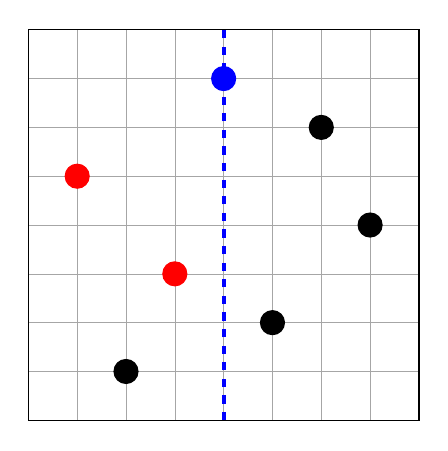
\begin{tikzpicture}[scale=0.62]
        \draw[very thin, gray!70] (0,0) grid (8,8);

        \draw[blue, dashed, line width=1.5pt] (4,0) -- (4,8);
        
        %\draw[red, line width=1.2pt] (1,5) rectangle (4,7);
        %\draw[red, line width=1.2pt] (3,3) rectangle (4,7);
        
        \filldraw[black] (2,1) circle (7pt);
        \filldraw[red] (3,3) circle (7pt);
        \filldraw[black] (5,2) circle (7pt);
        \filldraw[black] (7,4) circle (7pt);
        \filldraw[red] (1,5) circle (7pt);
        \filldraw[black] (6,6) circle (7pt);
        \filldraw[blue] (4,7) circle (7pt);
        \draw[black, line width=0.5pt] (0,0) rectangle (8,8);
    \end{tikzpicture}
    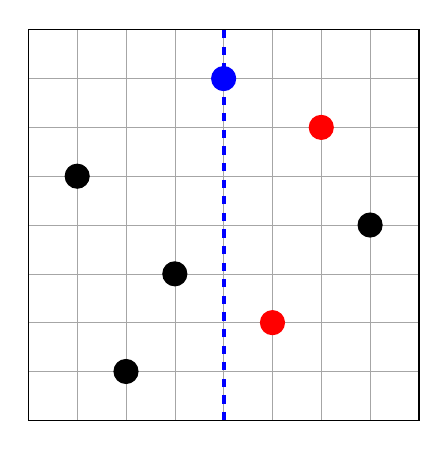
\begin{tikzpicture}[scale=0.62]
        \draw[very thin, gray!70] (0,0) grid (8,8);
        \draw[blue, dashed, line width=1.5pt] (4,0) -- (4,8);
        
        %\draw[red, line width=1.2pt] (5,2) rectangle (4,7);
        %\draw[red, line width=1.2pt] (6,6) rectangle (4,7);
        
        \filldraw[black] (2,1) circle (7pt);
        \filldraw[black] (3,3) circle (7pt);
        \filldraw[red] (5,2) circle (7pt);
        \filldraw[black] (7,4) circle (7pt);
        \filldraw[black] (1,5) circle (7pt);
        \filldraw[red] (6,6) circle (7pt);
        \filldraw[blue] (4,7) circle (7pt);
        \draw[black, line width=0.5pt] (0,0) rectangle (8,8);
    \end{tikzpicture}
    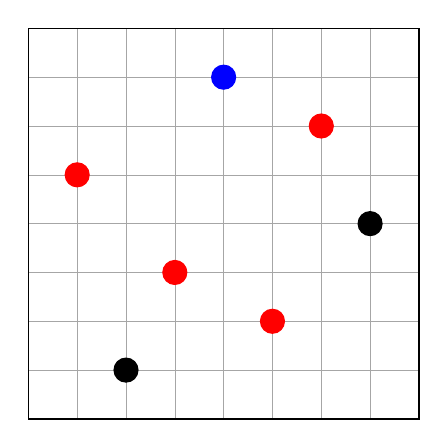
\begin{tikzpicture}[scale=0.62]
        \draw[very thin, gray!70] (0,0) grid (8,8);
        %\draw[blue, dashed, line width=1.5pt] (4,0) -- (4,8);
        
        \filldraw[black] (2,1) circle (7pt);
        \filldraw[red] (3,3) circle (7pt);
        \filldraw[red] (5,2) circle (7pt);
        \filldraw[black] (7,4) circle (7pt);
        \filldraw[red] (1,5) circle (7pt);
        \filldraw[red] (6,6) circle (7pt);
        \filldraw[blue] (4,7) circle (7pt);
        \draw[black, line width=0.5pt] (0,0) rectangle (8,8);
    \end{tikzpicture}
    %\caption{Nesta visão geométrica de uma sequência de acessos, está destacado de azul o ponto (4,7). À esquerda, estão destacados de vermelho os pontos do Funil esquerdo do ponto azul. Ao meio, estão destacados os pontos do Funil direito do ponto azul. À direita, estão destacados os pontos pertencentes ao funil do ponto azul.}
    \caption{O ponto (4,7) está destacado. À esquerda, os pontos vermelhos pertencem ao lado esquerdo do funil do ponto azul. Ao meio, os pontos vermelhos pertencem ao lado direito do funil do ponto azul. À direita, estão destacados de vermelho os pontos do funil do ponto azul, que são a união dos dois conjuntos anteriores.}
\label{fig:funil-apresentacao}
\end{figure}

A delimitação do funil para um ponto conta o número de intercalações entre o lado esquerdo e direito do funil. Assim, para cada ponto $p$ de $P$, definimos $f(P,p) = \emph{intercala}(F_E(P,p).y, F_D(P,p).y)$. A \textit{delimitação do funil} para uma sequência~$X$ de acessos é a somatória desse valor para todos os pontos da visão geométrica de $X$, ou seja, \Funil$(X) = \sum_{p \in P_X}{f(P_X,p)}$. Veja a Figura~\ref{fig:funil-execucao}.

Grosseiramente, $f(P,p)$ é o número de intercalações direita-esquerda dos pontos de $P$ abaixo de $p$, indo de cima para baixo, cujas $x$-coordenadas se aproximam da $x$-coordenada de $p$.

\begin{comment}
    \begin{figure}
        \centering
        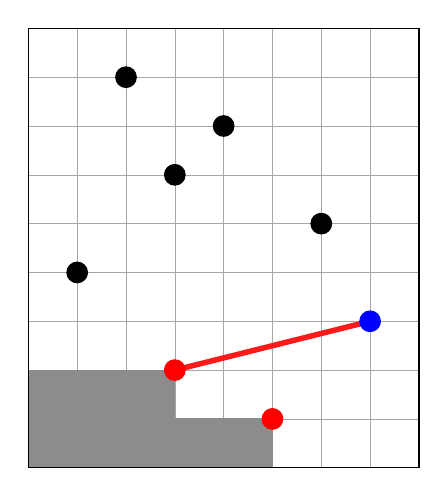
\begin{tikzpicture}[scale=0.62]
            \draw[very thin, gray!70] (0,0) grid (8,9);
            
            \draw[fill=gray!90, gray!90] (0,0) rectangle (3,2);
            \draw[fill=gray!90, gray!90] (1,0) rectangle (5,1);

            \draw[red!90, line width=2pt] (7,3) -- (3,2);  

            \filldraw[red] (5,1) circle (6pt);
            \filldraw[red] (3,2) circle (6pt);
            \filldraw[blue] (7,3) circle (6pt);
            \filldraw[black] (1,4) circle (6pt);
            \filldraw[black] (6,5) circle (6pt);
            \filldraw[black] (3,6) circle (6pt);
            \filldraw[black] (4,7) circle (6pt);
            \filldraw[black] (2,8) circle (6pt);


            %\node at (1,9.5) {\textbf{\Large E}};
            %\node at (2,8.5) {\textbf{\Large E}};
            %\node at (4,5.5) {\textbf{\Large E}};
            %\node at (5,1.5) {\textbf{\Large E}};

            %\node at (10,7.5) {\textbf{\Large D}};
            %\node at (8,6.5) {\textbf{\Large D}};
            %\node at (7,2.5) {\textbf{\Large D}};


            \draw[black, line width=0.5pt] (0,0) rectangle (8,9);
        \end{tikzpicture}
        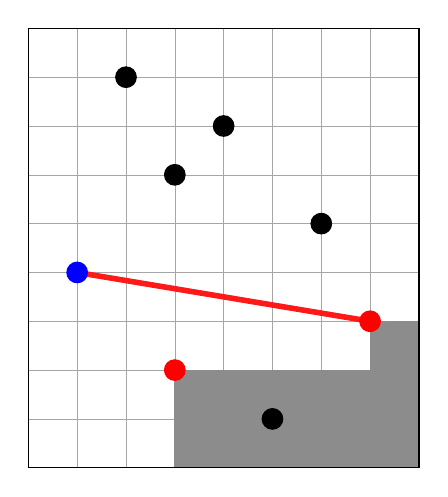
\begin{tikzpicture}[scale=0.62]
            \draw[very thin, gray!70] (0,0) grid (8,9);
            
            \draw[fill=gray!90, gray!90] (8,0) rectangle (3,2);
            \draw[fill=gray!90, gray!90] (8,0) rectangle (7,3);

            \draw[red!90, line width=2pt] (1,4) -- (7,3); 

            \filldraw[black] (5,1) circle (6pt);
            \filldraw[red] (3,2) circle (6pt);
            \filldraw[red] (7,3) circle (6pt);
            \filldraw[blue] (1,4) circle (6pt);
            \filldraw[black] (6,5) circle (6pt);
            \filldraw[black] (3,6) circle (6pt);
            \filldraw[black] (4,7) circle (6pt);
            \filldraw[black] (2,8) circle (6pt);


            %\node at (1,9.5) {\textbf{\Large E}};
            %\node at (2,8.5) {\textbf{\Large E}};
            %\node at (4,5.5) {\textbf{\Large E}};
            %\node at (5,1.5) {\textbf{\Large E}};

            %\node at (10,7.5) {\textbf{\Large D}};
            %\node at (8,6.5) {\textbf{\Large D}};
            %\node at (7,2.5) {\textbf{\Large D}};


            \draw[black, line width=0.5pt] (0,0) rectangle (8,9);
        \end{tikzpicture}
        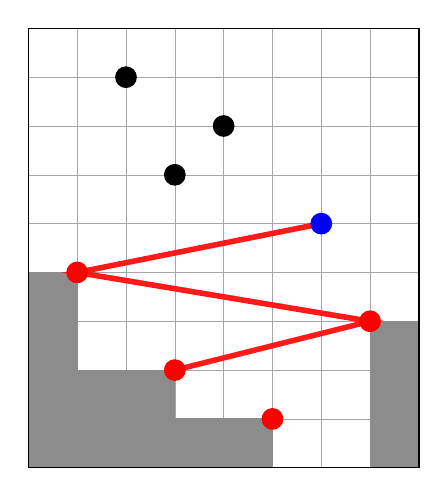
\begin{tikzpicture}[scale=0.62] %3
            \draw[very thin, gray!70] (0,0) grid (8,9);
            
            \draw[fill=gray!90, gray!90] (0,0) rectangle (5,1);
            \draw[fill=gray!90, gray!90] (0,0) rectangle (3,2);
            \draw[fill=gray!90, gray!90] (8,0) rectangle (7,3);
            \draw[fill=gray!90, gray!90] (0,0) rectangle (1,4);

            \draw[red!90, line width=2pt] (6,5) -- (1,4) -- (7,3) -- (3,2);

            \filldraw[red] (5,1) circle (6pt);
            \filldraw[red] (3,2) circle (6pt);
            \filldraw[red] (7,3) circle (6pt);
            \filldraw[red] (1,4) circle (6pt);
            \filldraw[blue] (6,5) circle (6pt);
            \filldraw[black] (3,6) circle (6pt);
            \filldraw[black] (4,7) circle (6pt);
            \filldraw[black] (2,8) circle (6pt);


            %\node at (1,9.5) {\textbf{\Large E}};
            %\node at (2,8.5) {\textbf{\Large E}};
            %\node at (4,5.5) {\textbf{\Large E}};
            %\node at (5,1.5) {\textbf{\Large E}};

            %\node at (10,7.5) {\textbf{\Large D}};
            %\node at (8,6.5) {\textbf{\Large D}};
            %\node at (7,2.5) {\textbf{\Large D}};


            \draw[black, line width=0.5pt] (0,0) rectangle (8,9);
        \end{tikzpicture}
        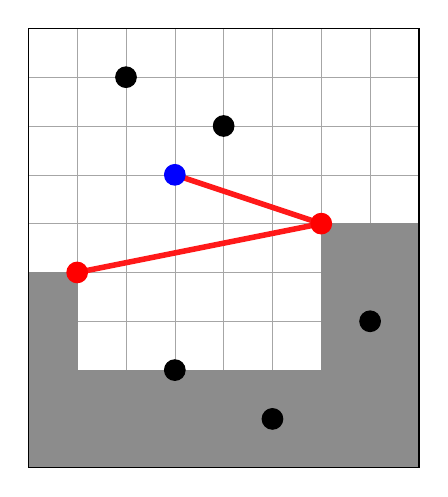
\begin{tikzpicture}[scale=0.62] %4
            \draw[very thin, gray!70] (0,0) grid (8,9);
            
            \draw[fill=gray!90, gray!90] (0,0) rectangle (1,4);
            \draw[fill=gray!90, gray!90] (8,0) rectangle (6,5);
            \draw[fill=gray!90, gray!90] (0,0) rectangle (3,2);
            \draw[fill=gray!90, gray!90] (8,0) rectangle (3,2);

            \draw[red!90, line width=2pt] (3,6) -- (6,5) -- (1,4);

            %\draw[fill=gray!90, gray!90] (10,7) rectangle (11,0);
            %\draw[fill=gray!90, gray!90] (8,6) rectangle (10,0);
            %\draw[fill=gray!90, gray!90] (7,2) rectangle (8,0);    

            \filldraw[black] (5,1) circle (6pt);
            \filldraw[black] (3,2) circle (6pt);
            \filldraw[black] (7,3) circle (6pt);
            \filldraw[red] (1,4) circle (6pt);
            \filldraw[red] (6,5) circle (6pt);
            \filldraw[blue] (3,6) circle (6pt);
            \filldraw[black] (4,7) circle (6pt);
            \filldraw[black] (2,8) circle (6pt);


            %\node at (1,9.5) {\textbf{\Large E}};
            %\node at (2,8.5) {\textbf{\Large E}};
            %\node at (4,5.5) {\textbf{\Large E}};
            %\node at (5,1.5) {\textbf{\Large E}};

            %\node at (10,7.5) {\textbf{\Large D}};
            %\node at (8,6.5) {\textbf{\Large D}};
            %\node at (7,2.5) {\textbf{\Large D}};


            \draw[black, line width=0.5pt] (0,0) rectangle (8,9);
        \end{tikzpicture}
        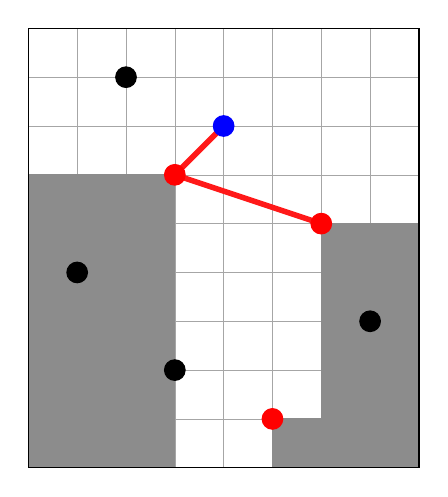
\begin{tikzpicture}[scale=0.62] %5
            \draw[very thin, gray!70] (0,0) grid (8,9);
            
            \draw[fill=gray!90, gray!90] (0,0) rectangle (3,6);
            \draw[fill=gray!90, gray!90] (8,0) rectangle (5,1);
            \draw[fill=gray!90, gray!90] (8,0) rectangle (6,5);
            %\draw[fill=gray!90, gray!90] (1,0) rectangle (2,8);
            %\draw[fill=gray!90, gray!90] (2,0) rectangle (4,5);
            %\draw[fill=gray!90, gray!90] (4,0) rectangle (5,1);

            \draw[red!90, line width=2pt] (4,7) -- (3,6) -- (6,5);
            %\draw[red!90, line width=2pt] (8,6) -- (4,5) -- (7,2) -- (5,1);

            %\draw[fill=gray!90, gray!90] (10,7) rectangle (11,0);
            %\draw[fill=gray!90, gray!90] (8,6) rectangle (10,0);
            %\draw[fill=gray!90, gray!90] (7,2) rectangle (8,0);    

            \filldraw[red] (5,1) circle (6pt);
            \filldraw[black] (3,2) circle (6pt);
            \filldraw[black] (7,3) circle (6pt);
            \filldraw[black] (1,4) circle (6pt);
            \filldraw[red] (6,5) circle (6pt);
            \filldraw[red] (3,6) circle (6pt);
            \filldraw[blue] (4,7) circle (6pt);
            \filldraw[black] (2,8) circle (6pt);


            %\node at (1,9.5) {\textbf{\Large E}};
            %\node at (2,8.5) {\textbf{\Large E}};
            %\node at (4,5.5) {\textbf{\Large E}};
            %\node at (5,1.5) {\textbf{\Large E}};

            %\node at (10,7.5) {\textbf{\Large D}};
            %\node at (8,6.5) {\textbf{\Large D}};
            %\node at (7,2.5) {\textbf{\Large D}};


            \draw[black, line width=0.5pt] (0,0) rectangle (8,9);
        \end{tikzpicture}
        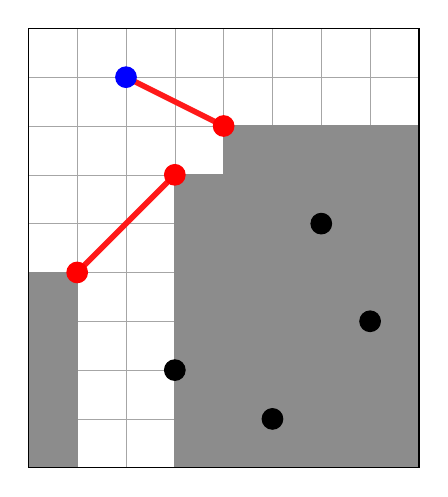
\begin{tikzpicture}[scale=0.62] %6
            \draw[very thin, gray!70] (0,0) grid (8,9);
            
            \draw[fill=gray!90, gray!90] (0,0) rectangle (1,4);
            \draw[fill=gray!90, gray!90] (8,0) rectangle (3,6);
            \draw[fill=gray!90, gray!90] (8,0) rectangle (4,7);

            \draw[red!90, line width=2pt] (2,8) -- (4,7);
            \draw[red!90, line width=2pt] (3,6) -- (1,4);

            \filldraw[black] (5,1) circle (6pt);
            \filldraw[black] (3,2) circle (6pt);
            \filldraw[black] (7,3) circle (6pt);
            \filldraw[red] (1,4) circle (6pt);
            \filldraw[black] (6,5) circle (6pt);
            \filldraw[red] (3,6) circle (6pt);
            \filldraw[red] (4,7) circle (6pt);
            \filldraw[blue] (2,8) circle (6pt);

            \draw[black, line width=0.5pt] (0,0) rectangle (8,9);
        \end{tikzpicture}
    \caption{Para a sequência de acessos $X = (5,3,7,1,3,4,2)$, o cálculo de $f(P_X,p)$ para todo $p \in P_X$ é o número de linhas vermelhas. Cada imagem representa o cálculo para o ponto azul, os pontos vermelhos são os pontos pertencentes ao funil do ponto azul e cada linha vermelha representa uma intercalação dos funis esquerdo-direto desse ponto. A imagem dos primeiros dois pontos foi omitida}
    \end{figure}
\end{comment}

\begin{figure}
    \centering
    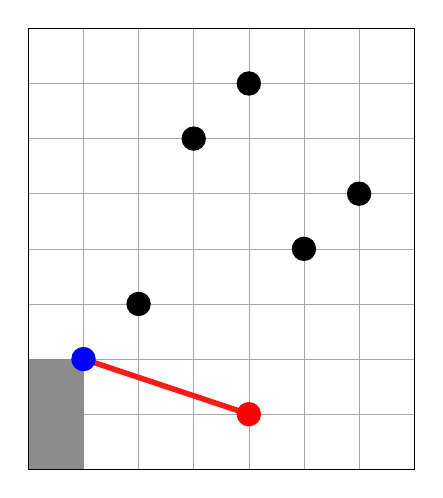
\begin{tikzpicture}[scale=0.7]
        \draw[very thin, gray!70] (0,0) grid (7,8);
        
        \draw[fill=gray!90, gray!90] (0,0) rectangle (1,2);

        \draw[red!90, line width=2pt] (1,2) -- (4,1);  

        \filldraw[red] (4,1) circle (6pt);
        \filldraw[blue] (1,2) circle (6pt);
        \filldraw[black] (2,3) circle (6pt);
        \filldraw[black] (5,4) circle (6pt);
        \filldraw[black] (6,5) circle (6pt);
        \filldraw[black] (3,6) circle (6pt);
        \filldraw[black] (4,7) circle (6pt);


        %\node at (1,9.5) {\textbf{\Large E}};
        %\node at (2,8.5) {\textbf{\Large E}};
        %\node at (4,5.5) {\textbf{\Large E}};
        %\node at (5,1.5) {\textbf{\Large E}};

        %\node at (10,7.5) {\textbf{\Large D}};
        %\node at (8,6.5) {\textbf{\Large D}};
        %\node at (7,2.5) {\textbf{\Large D}};


        \draw[black, line width=0.5pt] (0,0) rectangle (7,8);
    \end{tikzpicture}
    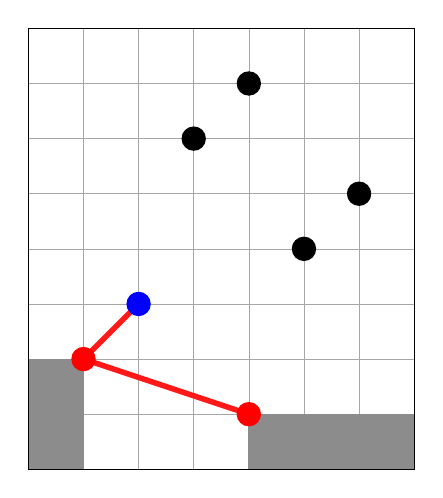
\begin{tikzpicture}[scale=0.7]
        \draw[very thin, gray!70] (0,0) grid (7,8);
        
        \draw[fill=gray!90, gray!90] (0,0) rectangle (1,2);
        \draw[fill=gray!90, gray!90] (7,0) rectangle (4,1);
        %\draw[fill=gray!90, gray!90] (1,0) rectangle (5,1);

        \draw[red!90, line width=2pt] (2,3) -- (1,2) -- (4,1);  

        \filldraw[red] (4,1) circle (6pt);
        \filldraw[red] (1,2) circle (6pt);
        \filldraw[blue] (2,3) circle (6pt);
        \filldraw[black] (5,4) circle (6pt);
        \filldraw[black] (6,5) circle (6pt);
        \filldraw[black] (3,6) circle (6pt);
        \filldraw[black] (4,7) circle (6pt);


        %\node at (1,9.5) {\textbf{\Large E}};
        %\node at (2,8.5) {\textbf{\Large E}};
        %\node at (4,5.5) {\textbf{\Large E}};
        %\node at (5,1.5) {\textbf{\Large E}};

        %\node at (10,7.5) {\textbf{\Large D}};
        %\node at (8,6.5) {\textbf{\Large D}};
        %\node at (7,2.5) {\textbf{\Large D}};


        \draw[black, line width=0.5pt] (0,0) rectangle (7,8);
    \end{tikzpicture}
    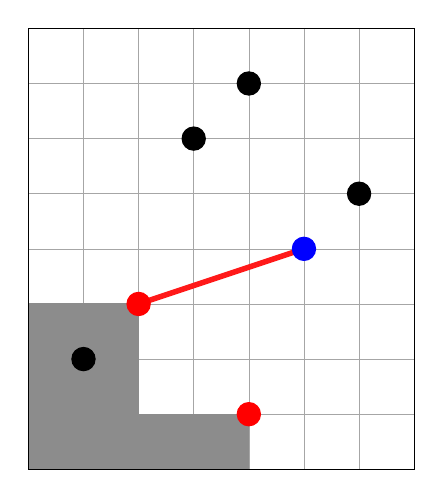
\begin{tikzpicture}[scale=0.7]
        \draw[very thin, gray!70] (0,0) grid (7,8);
        
        \draw[fill=gray!90, gray!90] (0,0) rectangle (4,1);
        \draw[fill=gray!90, gray!90] (0,0) rectangle (2,3);
        %\draw[fill=gray!90, gray!90] (1,0) rectangle (5,1);

        \draw[red!90, line width=2pt] (5,4) -- (2,3);  

        \filldraw[red] (4,1) circle (6pt);
        \filldraw[black] (1,2) circle (6pt);
        \filldraw[red] (2,3) circle (6pt);
        \filldraw[blue] (5,4) circle (6pt);
        \filldraw[black] (6,5) circle (6pt);
        \filldraw[black] (3,6) circle (6pt);
        \filldraw[black] (4,7) circle (6pt);


        %\node at (1,9.5) {\textbf{\Large E}};
        %\node at (2,8.5) {\textbf{\Large E}};
        %\node at (4,5.5) {\textbf{\Large E}};
        %\node at (5,1.5) {\textbf{\Large E}};

        %\node at (10,7.5) {\textbf{\Large D}};
        %\node at (8,6.5) {\textbf{\Large D}};
        %\node at (7,2.5) {\textbf{\Large D}};


        \draw[black, line width=0.5pt] (0,0) rectangle (7,8);
    \end{tikzpicture}
    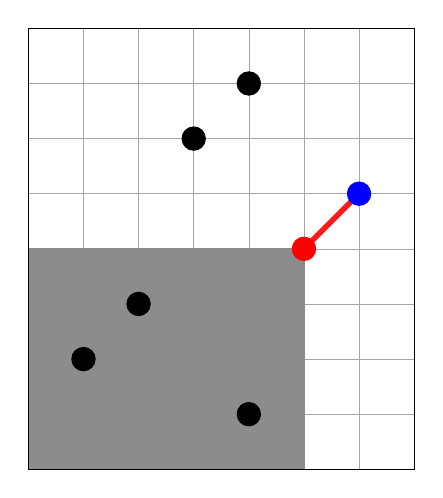
\begin{tikzpicture}[scale=0.7]
        \draw[very thin, gray!70] (0,0) grid (7,8);
        
        \draw[fill=gray!90, gray!90] (0,0) rectangle (5,4);
        %\draw[fill=gray!90, gray!90] (1,0) rectangle (5,1);

        \draw[red!90, line width=2pt] (6,5) -- (5,4);  

        \filldraw[black] (4,1) circle (6pt);
        \filldraw[black] (2,3) circle (6pt);
        \filldraw[black] (1,2) circle (6pt);
        \filldraw[red] (5,4) circle (6pt);
        \filldraw[blue] (6,5) circle (6pt);
        \filldraw[black] (3,6) circle (6pt);
        \filldraw[black] (4,7) circle (6pt);


        %\node at (1,9.5) {\textbf{\Large E}};
        %\node at (2,8.5) {\textbf{\Large E}};
        %\node at (4,5.5) {\textbf{\Large E}};
        %\node at (5,1.5) {\textbf{\Large E}};

        %\node at (10,7.5) {\textbf{\Large D}};
        %\node at (8,6.5) {\textbf{\Large D}};
        %\node at (7,2.5) {\textbf{\Large D}};


        \draw[black, line width=0.5pt] (0,0) rectangle (7,8);
    \end{tikzpicture}
    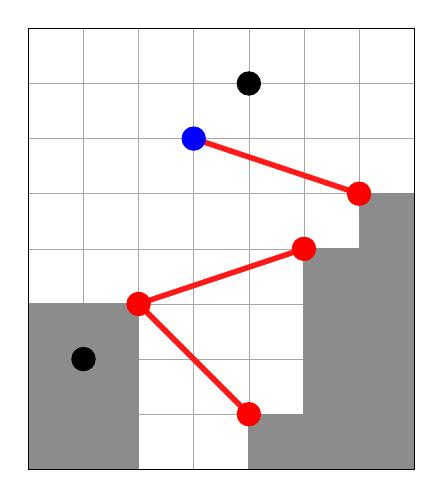
\begin{tikzpicture}[scale=0.7]
        \draw[very thin, gray!70] (0,0) grid (7,8);
        
        \draw[fill=gray!90, gray!90] (7,0) rectangle (6,5);
        \draw[fill=gray!90, gray!90] (7,0) rectangle (5,4);
        \draw[fill=gray!90, gray!90] (0,0) rectangle (2,3);
        \draw[fill=gray!90, gray!90] (7,0) rectangle (4,1);
        %\draw[fill=gray!90, gray!90] (1,0) rectangle (5,1);

        \draw[red!90, line width=2pt] (3,6) -- (6,5);  
        \draw[red!90, line width=2pt] (5,4) -- (2,3) -- (4,1);  

        \filldraw[red] (4,1) circle (6pt);
        \filldraw[red] (2,3) circle (6pt);
        \filldraw[black] (1,2) circle (6pt);
        \filldraw[red] (5,4) circle (6pt);
        \filldraw[red] (6,5) circle (6pt);
        \filldraw[blue] (3,6) circle (6pt);
        \filldraw[black] (4,7) circle (6pt);


        %\node at (1,9.5) {\textbf{\Large E}};
        %\node at (2,8.5) {\textbf{\Large E}};
        %\node at (4,5.5) {\textbf{\Large E}};
        %\node at (5,1.5) {\textbf{\Large E}};

        %\node at (10,7.5) {\textbf{\Large D}};
        %\node at (8,6.5) {\textbf{\Large D}};
        %\node at (7,2.5) {\textbf{\Large D}};


        \draw[black, line width=0.5pt] (0,0) rectangle (7,8);
    \end{tikzpicture}
    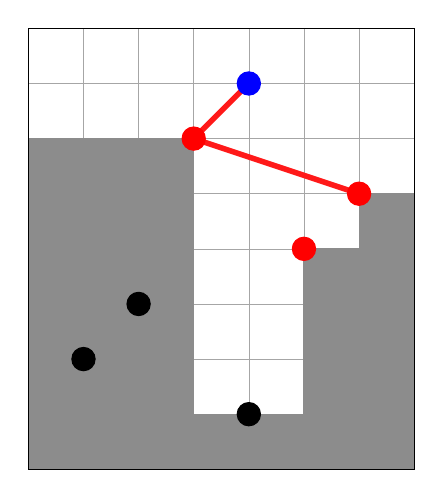
\begin{tikzpicture}[scale=0.7]
        \draw[very thin, gray!70] (0,0) grid (7,8);
        
        \draw[fill=gray!90, gray!90] (0,0) rectangle (3,6);
        \draw[fill=gray!90, gray!90] (7,0) rectangle (6,5);
        \draw[fill=gray!90, gray!90] (7,0) rectangle (5,4);
        \draw[fill=gray!90, gray!90] (0,0) rectangle (4,1);
        \draw[fill=gray!90, gray!90] (7,0) rectangle (4,1);

        \draw[red!90, line width=2pt] (4,7) -- (3,6) -- (6,5);  

        \filldraw[black] (4,1) circle (6pt);
        \filldraw[black] (2,3) circle (6pt);
        \filldraw[black] (1,2) circle (6pt);
        \filldraw[red] (5,4) circle (6pt);
        \filldraw[red] (6,5) circle (6pt);
        \filldraw[red] (3,6) circle (6pt);
        \filldraw[blue] (4,7) circle (6pt);


        %\node at (1,9.5) {\textbf{\Large E}};
        %\node at (2,8.5) {\textbf{\Large E}};
        %\node at (4,5.5) {\textbf{\Large E}};
        %\node at (5,1.5) {\textbf{\Large E}};

        %\node at (10,7.5) {\textbf{\Large D}};
        %\node at (8,6.5) {\textbf{\Large D}};
        %\node at (7,2.5) {\textbf{\Large D}};


        \draw[black, line width=0.5pt] (0,0) rectangle (7,8);
    \end{tikzpicture}    
    \caption{Para a sequência $X = (4,1,2,5,6,3,4)$ de acessos, o cálculo de $f(P_X,p)$ para todo $p \in P_X$ é o número de linhas vermelhas. Cada imagem representa o cálculo de $f(P_X,p)$ para o ponto azul $p$. Os pontos vermelhos são os pontos pertencentes ao funil de $p$ e cada linha vermelha representa uma intercalação dos lados esquerdo-direto do funil desse ponto. Para essa sequência de acessos, \Funil$(X) = 10$.}
\label{fig:funil-execucao}
\end{figure}

\section{Conjunto independente de retângulos a partir do funil}

%É possível encontrar um conjunto independente de retângulos associado a esta delimitação a partir do seguinte algoritmo: para cada ponto $p \in P_X$, trace um retângulo com vértices $p$ e $q$ para todo $q \in P_X$ associado à última ocorrência da string $E$ ou $D$ de cada bloco contíguo de $mix(F_E(P,p).y, F_D(P,p).y)$. Em outras palavaras, trace um retângulo com vértices em $p$ e $q$ para todo ponto $q$ que for o ponto mais alto do funil esquerdo ou do funil direito antes de uma intercalação.

%Note que todos os pares de ponto $(p,q)$ encontrados possuem o ponto $p$ como o ponto analisado e $q$ como pontos abaixo de $p$. Assim, por construção, todos os retângulos encontrados são distintos. Além disso, por definição, todos os pontos $q$ pertencentes ao funil do ponto $p$ possuem o $\{p,q\}$-retângulo arboreamente insatisfeito, logo o conjunto de retângulos encontrado é independente.

Nessa seção, mostraremos um algoritmo que encontra um conjunto independente $I$ de retângulos para $P_X$ a partir de uma sequência $X$ de acessos. Mostraremos que o conjunto de retângulos produzido pelo algoritmo tem \Funil$(X)$ retângulos. Como na Seção~\ref{sec:alt_com_ret}, o algoritmo encontrará pares de pontos de $P_X$ que representam retângulos.

O algoritmo inicializa $I$ como vazio e, para cada ponto $p \in P_X$, adiciona o par $(p,q)$ de pontos a $I$ para todo ponto $q \in P_X$ associado à última ocorrência de \textbf{E} ou \textbf{D} de cada bloco contíguo de $mix(F_E(P,p).y, F_D(P,p).y)$, como na Seção~\ref{sec:visao_geral}. Em outras palavras, o algoritmo inclui em $I$ todo par de pontos $(p,q)$ tal que $q$ é o ponto mais alto do lado esquerdo ou do lado direito do funil de $p$ antes de uma intercalação. Veja a Figura~\ref{fig:retangulos_no_funil}.

%Mostraremos que $I$ representa um conjunto independente de retângulos de tamanho Funil$(X)$. 
Note que todos os pares $(p,q)$ de pontos adicionados a $I$ possuem o ponto $p$ como o ponto analisado e $q$ como ponto abaixo de $p$. Assim, por construção, são encontrados $\Funil(X)$ pares de pontos distintos. Além disso, por definição, todos os pontos $q$ pertencentes ao funil de um ponto $p$ possuem o $\{p,q\}$-retângulo arboreamente insatisfeito, logo o conjunto de retângulos encontrado é independente.

\begin{figure}
    \centering
    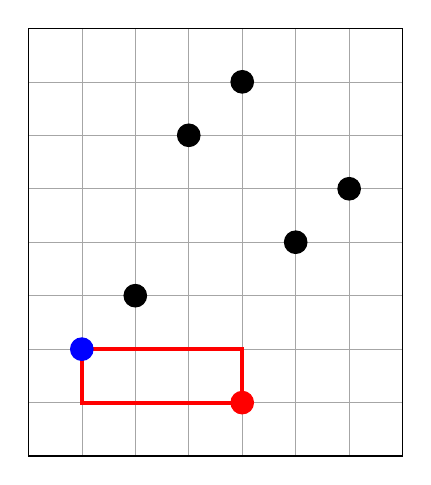
\begin{tikzpicture}[scale=0.679]
        \draw[very thin, gray!70] (0,0) grid (7,8);
        
        %\draw[fill=gray!90, gray!90] (0,0) rectangle (1,2);

        \draw[red, line width=1.5pt] (1,2) rectangle (4,1);

        \filldraw[red] (4,1) circle (6pt);
        \filldraw[blue] (1,2) circle (6pt);
        \filldraw[black] (2,3) circle (6pt);
        \filldraw[black] (5,4) circle (6pt);
        \filldraw[black] (6,5) circle (6pt);
        \filldraw[black] (3,6) circle (6pt);
        \filldraw[black] (4,7) circle (6pt);

        \draw[black, line width=0.5pt] (0,0) rectangle (7,8);
    \end{tikzpicture}
    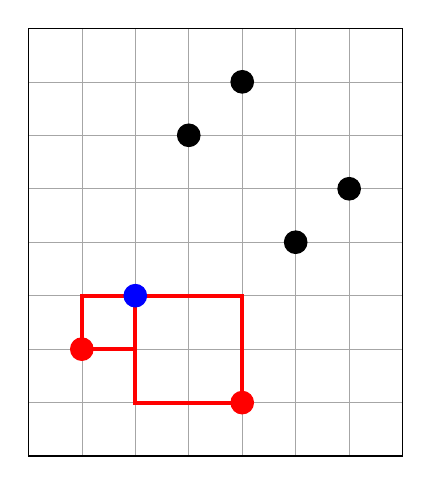
\begin{tikzpicture}[scale=0.679]
        \draw[very thin, gray!70] (0,0) grid (7,8);
        
        %\draw[fill=gray!90, gray!90] (0,0) rectangle (1,2);
        %\draw[fill=gray!90, gray!90] (7,0) rectangle (4,1);
        %\draw[fill=gray!90, gray!90] (1,0) rectangle (5,1);
        \draw[red, line width=1.5pt] (1,2) rectangle (2,3);
        \draw[red, line width=1.5pt] (4,1) rectangle (2,3);

        %\draw[red!90, line width=2pt] (2,3) -- (1,2) -- (4,1);  

        \filldraw[red] (4,1) circle (6pt);
        \filldraw[red] (1,2) circle (6pt);
        \filldraw[blue] (2,3) circle (6pt);
        \filldraw[black] (5,4) circle (6pt);
        \filldraw[black] (6,5) circle (6pt);
        \filldraw[black] (3,6) circle (6pt);
        \filldraw[black] (4,7) circle (6pt);

        \draw[black, line width=0.5pt] (0,0) rectangle (7,8);
    \end{tikzpicture}
    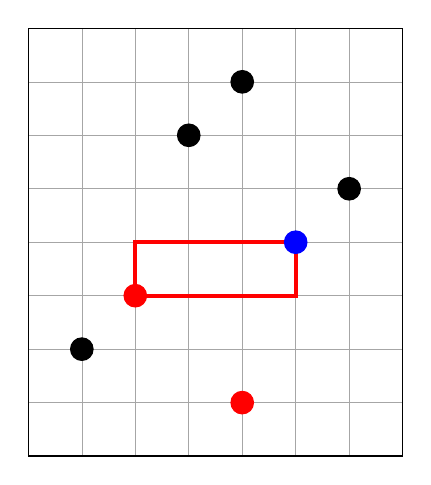
\begin{tikzpicture}[scale=0.679]
        \draw[very thin, gray!70] (0,0) grid (7,8);
        
        %\draw[fill=gray!90, gray!90] (0,0) rectangle (4,1);
        %\draw[fill=gray!90, gray!90] (0,0) rectangle (2,3);
        %\draw[fill=gray!90, gray!90] (1,0) rectangle (5,1);

        \draw[red, line width=1.5pt] (5,4) rectangle (2,3);

        %\draw[red!90, line width=2pt] (5,4) -- (2,3);  

        \filldraw[red] (4,1) circle (6pt);
        \filldraw[black] (1,2) circle (6pt);
        \filldraw[red] (2,3) circle (6pt);
        \filldraw[blue] (5,4) circle (6pt);
        \filldraw[black] (6,5) circle (6pt);
        \filldraw[black] (3,6) circle (6pt);
        \filldraw[black] (4,7) circle (6pt);

        \draw[black, line width=0.5pt] (0,0) rectangle (7,8);
    \end{tikzpicture}
    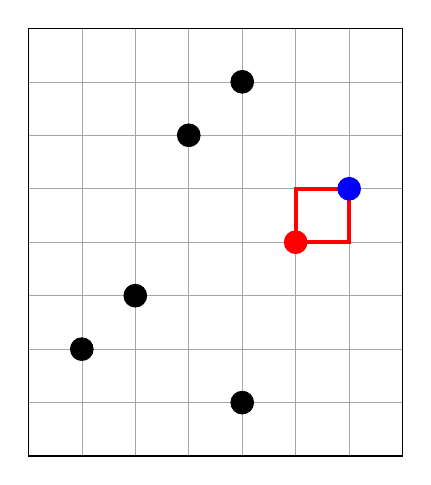
\begin{tikzpicture}[scale=0.679]
        \draw[very thin, gray!70] (0,0) grid (7,8);
        
        %\draw[fill=gray!90, gray!90] (0,0) rectangle (5,4);
        %\draw[fill=gray!90, gray!90] (1,0) rectangle (5,1);

        \draw[red, line width=1.5pt] (6,5) rectangle (5,4);

        %\draw[red!90, line width=2pt] (6,5) -- (5,4);  

        \filldraw[black] (4,1) circle (6pt);
        \filldraw[black] (2,3) circle (6pt);
        \filldraw[black] (1,2) circle (6pt);
        \filldraw[red] (5,4) circle (6pt);
        \filldraw[blue] (6,5) circle (6pt);
        \filldraw[black] (3,6) circle (6pt);
        \filldraw[black] (4,7) circle (6pt);

        \draw[black, line width=0.5pt] (0,0) rectangle (7,8);
    \end{tikzpicture}
    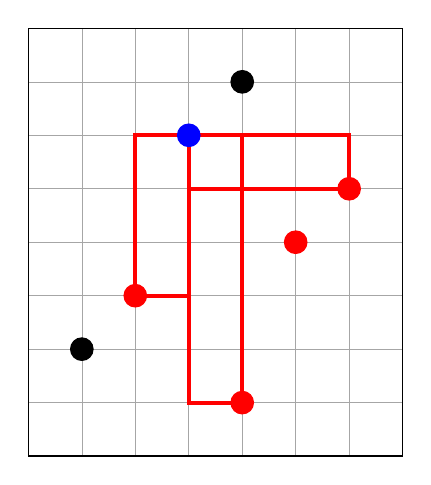
\begin{tikzpicture}[scale=0.679]
        \draw[very thin, gray!70] (0,0) grid (7,8);
        
        %\draw[fill=gray!90, gray!90] (7,0) rectangle (6,5);
        %\draw[fill=gray!90, gray!90] (7,0) rectangle (5,4);
        %\draw[fill=gray!90, gray!90] (0,0) rectangle (2,3);
        %\draw[fill=gray!90, gray!90] (7,0) rectangle (4,1);
        %\draw[fill=gray!90, gray!90] (1,0) rectangle (5,1);
        \draw[red, line width=1.5pt] (3,6) rectangle (6,5);
        \draw[red, line width=1.5pt] (3,6) rectangle (2,3);
        \draw[red, line width=1.5pt] (3,6) rectangle (4,1);

        %\draw[red!90, line width=2pt] (3,6) -- (6,5);  
        %draw[red!90, line width=2pt] (5,4) -- (2,3) -- (4,1);  

        \filldraw[red] (4,1) circle (6pt);
        \filldraw[red] (2,3) circle (6pt);
        \filldraw[black] (1,2) circle (6pt);
        \filldraw[red] (5,4) circle (6pt);
        \filldraw[red] (6,5) circle (6pt);
        \filldraw[blue] (3,6) circle (6pt);
        \filldraw[black] (4,7) circle (6pt);

        \draw[black, line width=0.5pt] (0,0) rectangle (7,8);
    \end{tikzpicture}
    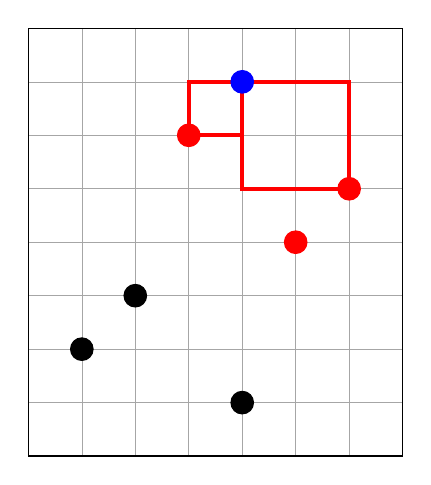
\begin{tikzpicture}[scale=0.679]
        \draw[very thin, gray!70] (0,0) grid (7,8);
        
        %\draw[fill=gray!90, gray!90] (0,0) rectangle (3,6);
        %\draw[fill=gray!90, gray!90] (7,0) rectangle (6,5);
        %\draw[fill=gray!90, gray!90] (7,0) rectangle (5,4);
        %\draw[fill=gray!90, gray!90] (0,0) rectangle (4,1);
        %\draw[fill=gray!90, gray!90] (7,0) rectangle (4,1);

        \draw[red, line width=1.5pt] (4,7) rectangle (3,6);
        \draw[red, line width=1.5pt] (4,7) rectangle (6,5);
        %\draw[red!90, line width=2pt] (4,7) -- (3,6) -- (6,5);  

        \filldraw[black] (4,1) circle (6pt);
        \filldraw[black] (2,3) circle (6pt);
        \filldraw[black] (1,2) circle (6pt);
        \filldraw[red] (5,4) circle (6pt);
        \filldraw[red] (6,5) circle (6pt);
        \filldraw[red] (3,6) circle (6pt);
        \filldraw[blue] (4,7) circle (6pt);

        \draw[black, line width=0.5pt] (0,0) rectangle (7,8);
    \end{tikzpicture}    
    \caption{Para a sequência de acessos $X = (4,1,2,5,6,3,4)$. Para cada ponto azul, está destacado o conjunto independente de retângulos que será incluído em $I$ pelo algoritmo, referente à delimitação do funil para aquele ponto. Perceba que nem todos os pontos do funil do ponto analisado são incluídos. Comparando com a Figura~\ref{fig:funil-execucao}, é fácil notar que o tamanho do conjunto de retângulos final é exatamente \Funil$(X)$.}
\label{fig:retangulos_no_funil}
\end{figure}

\section{Sequência bit-reversa}

Para evidenciar como as delimitações propostas por Wilber podem ser uma ferramenta poderosa para analisar sequências de acessos, mostraremos uma sequência que é sempre custosa, independente do algoritmo de busca. 

Nesta seção, excepcionalmente, consideraremos que as ABBs contêm as chaves de $0$ a $n-1$. Essa consideração será útil para maior simplificação das análises, porém não é necessária para o estudo abaixo. 

Definimos a \textit{sequência bit-reversa} de $0$ a $n-1$ como a contagem de $0$ a $n-1$ em binário e depois a sua leitura de trás pra frente, ou seja, leia os bits de cada número da direita para a esquerda. Veja a Figura~\ref{fig:sequencia}.

\begin{figure}
    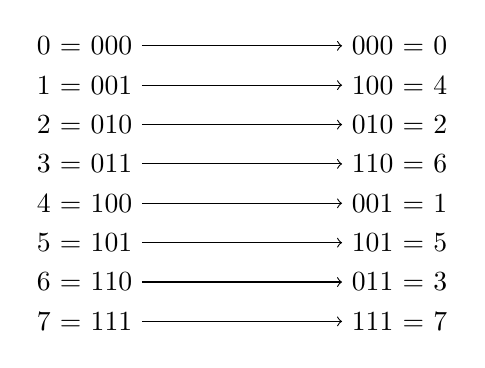
\begin{tikzpicture}
        \node (a) at (0, 0) {0 = 000};
        \node (b) at (0, -0.5) {1 = 001};
        \node (c) at (0, -1) {2 = 010};
        \node (d) at (0, -1.5) {3 = 011};
        \node (e) at (0, -2) {4 = 100};
        \node (f) at (0, -2.5) {5 = 101};
        \node (g) at (0, -3) {6 = 110};
        \node (h) at (0, -3.5) {7 = 111};

        \node (a') at (4, 0) {000 = 0};
        \node (b') at (4, -0.5) {100 = 4};
        \node (c') at (4, -1) {010 = 2};
        \node (d') at (4, -1.5) {110 = 6};
        \node (e') at (4, -2) {001 = 1};
        \node (f') at (4, -2.5) {101 = 5};
        \node (g') at (4, -3) {011 = 3};
        \node (h') at (4, -3.5) {111 = 7};

        \draw[->] (a) -- (a');
        \draw[->] (b) -- (b');
        \draw[->] (c) -- (c');
        \draw[->] (d) -- (d');
        \draw[->] (e) -- (e');
        \draw[->] (f) -- (f');
        \draw[->] (g) -- (g');
        \draw[->] (h) -- (h');
    \end{tikzpicture}
    \caption{Sequência bit-reversa para $n = 8$. A coluna da esquerda mostra a contagem de $0$ a $n - 1$ em binário e a  coluna da direita mostra a leitura desses números em base 2 de trás para frente, ou seja, considerando os bits da direita para a esquerda.}
\label{fig:sequencia}
\end{figure}

É bastante útil entender como um algoritmo de busca se comporta nas sequências de acessos em uma ABB completa fixa. Uma maneira de visualizar as buscas em binário dentro de uma ABB completa fixa é imaginar que os ponteiros representam um bit e a busca em binário dentro da ABB é a sequência de ponteiros, que com seus bits concatenados, resultam no número buscado. Veja a Figura~\ref{fig:abb-numerada}.

\begin{figure}
    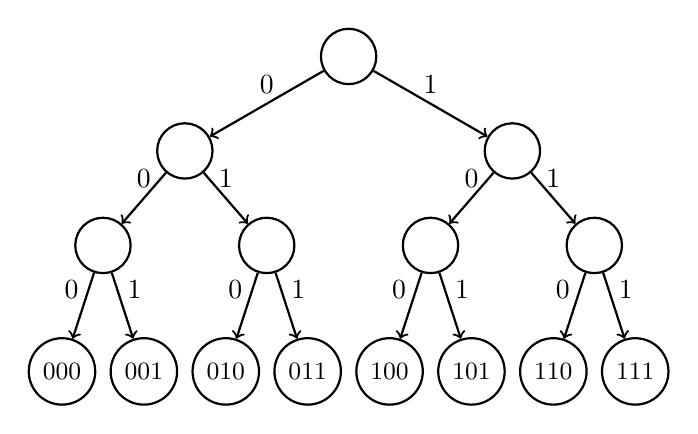
\begin{tikzpicture}[scale=0.8,
        node/.style={circle,draw,minimum size=2em, thick, font=\large},
        nodeGray/.style={circle,draw,minimum size=2em, thick, font=\large, fill=gray!55}]
        
        \node[node] (H) at (0,0) {};
        \node[node] (D) at (-2.6,-1.5) {};
        \node[node] (B) at (-3.9,-3) {};
        \node[node] (A) at (-4.55,-5) {\small$000$};
        \node[node] (C) at (-3.25,-5) {\small$001$};
        \node[node] (F) at (-1.3,-3) {};
        \node[node] (E) at (-1.95,-5) {\small$010$};
        \node[node] (G) at (-0.65,-5) {\small$011$};


        \node[node] (L) at (2.6,-1.5) {};
        \node[node] (J) at (3.9,-3) {};
        \node[node] (I) at (4.55,-5) {\small$111$};
        \node[node] (K) at (3.25,-5) {\small$110$};
        \node[node] (N) at (1.3,-3) {};
        \node[node] (M) at (1.95,-5) {\small$101$};
        \node[node] (O) at (0.65,-5) {\small$100$};
        
        \draw[thick, ->] (H) -- (D) node[midway, above] {$0$};
        \draw[thick, ->] (H) -- (L) node[midway, above] {$1$};
        \draw[thick, ->] (D) -- (B) node[midway, above] {$0$};
        \draw[thick, ->] (D) -- (F) node[midway, above] {$1$};
        \draw[thick, ->] (B) -- (A) node[near start, left] {$0$};
        \draw[thick, ->] (B) -- (C) node[near start, right] {$1$};
        \draw[thick, ->] (F) -- (E) node[near start, left] {$0$};
        \draw[thick, ->] (F) -- (G) node[near start, right] {$1$};

        \draw[thick, ->] (L) -- (J) node[midway, above] {$1$};
        \draw[thick, ->] (L) -- (N) node[midway, above] {$0$};
        \draw[thick, ->] (J) -- (I) node[near start, right] {$1$};
        \draw[thick, ->] (J) -- (K) node[near start, left] {$0$};
        \draw[thick, ->] (N) -- (M) node[near start, right] {$1$};
        \draw[thick, ->] (N) -- (O) node[near start, left] {$0$};
    \end{tikzpicture}
    \caption{ABB completa de 8 folhas com uma representação binária.}
\label{fig:abb-numerada}
\end{figure}

Como estamos lendo os bits de trás para frente, sabemos que a característica do contador binário se mantém porém com os bits ao contrário. Assim, sabemos que essa sequência tem a propriedade que o maior bit se altera em todo incremento do número, o segundo maior bit se altera em metade dos incrementos, o terceiro maior bit se altera em um quarto dos incrementos e o $i$-ésimo bit se altera em $2^{i - 1}$ dos incrementos.

Voltando ao contexto de ABBs, as alterações dos bits descritas acima implicam que cada busca começa indo por uma subárvore diferente, tanto na raiz como nos nós intermediários. Assim, como sabemos que as alternâncias começam pela esquerda por esta ser a ordem na contagem, deduzimos que para qualquer nó intermediário, a $j$-ésima busca em um de seus descendentes entrará na sua subárvore esquerda se $j$ for ímpar e na sua subárvore direita se $j$ for par.

A princípio essa informação não parece tão poderosa, porém relembremos como funciona a delimitação da alternância. Para qualquer ABB fixa com as chaves nas folhas, a somatória do número de intercalações esquerda-direita de todos os nós intermediários dessa ABB é uma delimitação inferior no custo de executar essa sequência de acessos dentro do modelo de computação adotado. Assim, como notado anteriormente, nunca há duas buscas consecutivas na mesma subárvore: todas as buscas se alternam em todos os nós. Portanto, sabemos que nenhum ponteiro de filho preferido será percorrido durante as buscas dessa sequência. Assim, essa sequência maximiza a delimitação da alternância.

Na ABB completa com $n$ folhas, cada folha tem altura $\lg n$. Então, sabemos que cada simulação de busca na ABB completa fixa acarretará em $\lg n$ alternâncias/alterações em ponteiros de filho preferido, e assim para uma sequência bit-reversa $X$ de acessos com $m$ buscas, \Alt$_\cT(X) = m \cdot \lg n$ para a árvore completa $\cT$ com $n$ folhas. Assim, sabemos que $\OPT(X) \geq m \cdot \lg n$.

Esse resultado é particularmente especial, pois nos mostra que a melhor maneira de executar todos os acessos dessa sequência vai ter custo maior ou igual a $m \cdot \lg n$, ou em média, $\lg n$ por busca. Essa é a delimitação trivial de árvores binárias de busca balanceadas como a árvore rubro-negra ou a AVL. Em outras palavras, essa sequência é tão cara no modelo de computação que não existe nenhuma maneira de melhorar seu custo acima da delimitação trivial, e assim, qualquer ABB balanceada com custo $\Oh(\lg n)$ por busca tem custo assintoticamente proporcional ao ótimo nessas sequências.

Por fim, vale a pena relembrar que essa sequência também é importante para as delimitações da eficiência do algoritmo guloso futurista. Como citado anteriormente, o pior caso conhecido do guloso futurista é buscar a sequência bit-reversa uma vez e depois seguir a sequência apenas buscando as folhas da ABB.

Note que esse caso é ruim, pois os nós intermediários se mantêm no caminho das folhas e não permitem que o algoritmo traga as folhas para perto da raiz. Assim, todas as buscas visitam uma série de nós desnecessários e acarretam em um custo de $\OPT(X) + \Oh(m)$. Veja a Figura~\ref{fig:GreedyFuture-bit-reversal}.

\begin{figure}
    \centering
    
    \begin{tikzpicture}[scale=0.34]
        \draw[very thin, gray] (0,0) grid (8,12);
        
        \draw[teste, very thick] (0,2) -- (8,2);

        \filldraw[black] (4,1) circle (8pt);
        \filldraw[black] (2,2) circle (8pt);
        \filldraw[red] (4,2) circle (8pt);
        \filldraw[black] (6,3) circle (8pt);
        \filldraw[black] (1,4) circle (8pt);
        \filldraw[black] (3,5) circle (8pt);
        \filldraw[black] (5,6) circle (8pt);
        \filldraw[black] (7,7) circle (8pt);
        \filldraw[black] (1,8) circle (8pt);
        \filldraw[black] (3,9) circle (8pt);
        \filldraw[black] (5,10) circle (8pt);
        \filldraw[black] (7,11) circle (8pt);
        \draw[black, line width=0.5pt] (0,0) rectangle (8,12);
    \end{tikzpicture}
    \begin{tikzpicture}[scale=0.34]
        \draw[very thin, gray] (0,0) grid (8,12);
        
        \draw[teste, very thick] (0,3) -- (8,3);

        \filldraw[black] (4,1) circle (8pt);
        \filldraw[black] (2,2) circle (8pt);
        \filldraw[red] (4,2) circle (8pt);
        \filldraw[black] (6,3) circle (8pt);
        \filldraw[red] (4,3) circle (8pt);
        \filldraw[black] (1,4) circle (8pt);
        \filldraw[black] (3,5) circle (8pt);
        \filldraw[black] (5,6) circle (8pt);
        \filldraw[black] (7,7) circle (8pt);
        \filldraw[black] (1,8) circle (8pt);
        \filldraw[black] (3,9) circle (8pt);
        \filldraw[black] (5,10) circle (8pt);
        \filldraw[black] (7,11) circle (8pt);
        \draw[black, line width=0.5pt] (0,0) rectangle (8,12);
    \end{tikzpicture}
    \begin{tikzpicture}[scale=0.34]
        \draw[very thin, gray] (0,0) grid (8,12);
        
        \draw[teste, very thick] (0,4) -- (8,4);

        \filldraw[black] (4,1) circle (8pt);
        \filldraw[black] (2,2) circle (8pt);
        \filldraw[red] (4,2) circle (8pt);
        \filldraw[black] (6,3) circle (8pt);
        \filldraw[red] (4,3) circle (8pt);
        \filldraw[black] (1,4) circle (8pt);
        \filldraw[red] (2,4) circle (8pt);
        \filldraw[red] (4,4) circle (8pt);
        \filldraw[black] (3,5) circle (8pt);
        \filldraw[black] (5,6) circle (8pt);
        \filldraw[black] (7,7) circle (8pt);
        \filldraw[black] (1,8) circle (8pt);
        \filldraw[black] (3,9) circle (8pt);
        \filldraw[black] (5,10) circle (8pt);
        \filldraw[black] (7,11) circle (8pt);
        \draw[black, line width=0.5pt] (0,0) rectangle (8,12);
    \end{tikzpicture}
    \begin{tikzpicture}[scale=0.34]
        \draw[very thin, gray] (0,0) grid (8,12);
        
        \draw[teste, very thick] (0,5) -- (8,5);

        \filldraw[black] (4,1) circle (8pt);
        \filldraw[black] (2,2) circle (8pt);
        \filldraw[red] (4,2) circle (8pt);
        \filldraw[black] (6,3) circle (8pt);
        \filldraw[red] (4,3) circle (8pt);
        \filldraw[black] (1,4) circle (8pt);
        \filldraw[red] (2,4) circle (8pt);
        \filldraw[red] (4,4) circle (8pt);
        \filldraw[black] (3,5) circle (8pt);
        \filldraw[red] (2,5) circle (8pt);
        \filldraw[red] (4,5) circle (8pt);
        \filldraw[black] (5,6) circle (8pt);
        \filldraw[black] (7,7) circle (8pt);
        \filldraw[black] (1,8) circle (8pt);
        \filldraw[black] (3,9) circle (8pt);
        \filldraw[black] (5,10) circle (8pt);
        \filldraw[black] (7,11) circle (8pt);
        \draw[black, line width=0.5pt] (0,0) rectangle (8,12);
    \end{tikzpicture}
    \begin{tikzpicture}[scale=0.34]
        \draw[very thin, gray] (0,0) grid (8,12);
        
        \draw[teste, very thick] (0,6) -- (8,6);

        \filldraw[black] (4,1) circle (8pt);
        \filldraw[black] (2,2) circle (8pt);
        \filldraw[red] (4,2) circle (8pt);
        \filldraw[black] (6,3) circle (8pt);
        \filldraw[red] (4,3) circle (8pt);
        \filldraw[black] (1,4) circle (8pt);
        \filldraw[red] (2,4) circle (8pt);
        \filldraw[red] (4,4) circle (8pt);
        \filldraw[black] (3,5) circle (8pt);
        \filldraw[red] (2,5) circle (8pt);
        \filldraw[red] (4,5) circle (8pt);
        \filldraw[red] (4,6) circle (8pt);
        \filldraw[black] (5,6) circle (8pt);
        \filldraw[red] (6,6) circle (8pt);
        \filldraw[black] (7,7) circle (8pt);
        \filldraw[black] (1,8) circle (8pt);
        \filldraw[black] (3,9) circle (8pt);
        \filldraw[black] (5,10) circle (8pt);
        \filldraw[black] (7,11) circle (8pt);
        \draw[black, line width=0.5pt] (0,0) rectangle (8,12);
    \end{tikzpicture}
    \\
    \begin{tikzpicture}[scale=0.34]
        \draw[very thin, gray] (0,0) grid (8,12);
        
        \draw[teste, very thick] (0,7) -- (8,7);

        \filldraw[black] (4,1) circle (8pt);
        \filldraw[black] (2,2) circle (8pt);
        \filldraw[red] (4,2) circle (8pt);
        \filldraw[black] (6,3) circle (8pt);
        \filldraw[red] (4,3) circle (8pt);
        \filldraw[black] (1,4) circle (8pt);
        \filldraw[red] (2,4) circle (8pt);
        \filldraw[red] (4,4) circle (8pt);
        \filldraw[black] (3,5) circle (8pt);
        \filldraw[red] (2,5) circle (8pt);
        \filldraw[red] (4,5) circle (8pt);
        \filldraw[red] (4,6) circle (8pt);
        \filldraw[black] (5,6) circle (8pt);
        \filldraw[red] (6,6) circle (8pt);
        \filldraw[red] (6,7) circle (8pt);
        \filldraw[black] (7,7) circle (8pt);
        \filldraw[black] (1,8) circle (8pt);
        \filldraw[black] (3,9) circle (8pt);
        \filldraw[black] (5,10) circle (8pt);
        \filldraw[black] (7,11) circle (8pt);
        \draw[black, line width=0.5pt] (0,0) rectangle (8,12);
    \end{tikzpicture}
    \begin{tikzpicture}[scale=0.34]
        \draw[very thin, gray] (0,0) grid (8,12);
        
        \draw[teste, very thick] (0,8) -- (8,8);

        \filldraw[black] (4,1) circle (8pt);
        \filldraw[black] (2,2) circle (8pt);
        \filldraw[red] (4,2) circle (8pt);
        \filldraw[black] (6,3) circle (8pt);
        \filldraw[red] (4,3) circle (8pt);
        \filldraw[black] (1,4) circle (8pt);
        \filldraw[red] (2,4) circle (8pt);
        \filldraw[red] (4,4) circle (8pt);
        \filldraw[black] (3,5) circle (8pt);
        \filldraw[red] (2,5) circle (8pt);
        \filldraw[red] (4,5) circle (8pt);
        \filldraw[red] (4,6) circle (8pt);
        \filldraw[black] (5,6) circle (8pt);
        \filldraw[red] (6,6) circle (8pt);
        \filldraw[red] (6,7) circle (8pt);
        \filldraw[black] (7,7) circle (8pt);
        \filldraw[black] (1,8) circle (8pt);
        \filldraw[red] (2,8) circle (8pt);
        \filldraw[red] (4,8) circle (8pt);
        \filldraw[red] (6,8) circle (8pt);
        \filldraw[black] (3,9) circle (8pt);
        \filldraw[black] (5,10) circle (8pt);
        \filldraw[black] (7,11) circle (8pt);
        \draw[black, line width=0.5pt] (0,0) rectangle (8,12);
    \end{tikzpicture}
    \begin{tikzpicture}[scale=0.34]
        \draw[very thin, gray] (0,0) grid (8,12);
        
        \draw[teste, very thick] (0,9) -- (8,9);

        \filldraw[black] (4,1) circle (8pt);
        \filldraw[black] (2,2) circle (8pt);
        \filldraw[red] (4,2) circle (8pt);
        \filldraw[black] (6,3) circle (8pt);
        \filldraw[red] (4,3) circle (8pt);
        \filldraw[black] (1,4) circle (8pt);
        \filldraw[red] (2,4) circle (8pt);
        \filldraw[red] (4,4) circle (8pt);
        \filldraw[black] (3,5) circle (8pt);
        \filldraw[red] (2,5) circle (8pt);
        \filldraw[red] (4,5) circle (8pt);
        \filldraw[red] (4,6) circle (8pt);
        \filldraw[black] (5,6) circle (8pt);
        \filldraw[red] (6,6) circle (8pt);
        \filldraw[red] (6,7) circle (8pt);
        \filldraw[black] (7,7) circle (8pt);
        \filldraw[black] (1,8) circle (8pt);
        \filldraw[red] (2,8) circle (8pt);
        \filldraw[red] (4,8) circle (8pt);
        \filldraw[red] (6,8) circle (8pt);
        \filldraw[black] (3,9) circle (8pt);
        \filldraw[red] (2,9) circle (8pt);
        \filldraw[red] (4,9) circle (8pt);
        \filldraw[black] (5,10) circle (8pt);
        \filldraw[black] (7,11) circle (8pt);
        \draw[black, line width=0.5pt] (0,0) rectangle (8,12);
    \end{tikzpicture}
    \begin{tikzpicture}[scale=0.34]
        \draw[very thin, gray] (0,0) grid (8,12);
        
        \draw[teste, very thick] (0,10) -- (8,10);

        \filldraw[black] (4,1) circle (8pt);
        \filldraw[black] (2,2) circle (8pt);
        \filldraw[red] (4,2) circle (8pt);
        \filldraw[black] (6,3) circle (8pt);
        \filldraw[red] (4,3) circle (8pt);
        \filldraw[black] (1,4) circle (8pt);
        \filldraw[red] (2,4) circle (8pt);
        \filldraw[red] (4,4) circle (8pt);
        \filldraw[black] (3,5) circle (8pt);
        \filldraw[red] (2,5) circle (8pt);
        \filldraw[red] (4,5) circle (8pt);
        \filldraw[red] (4,6) circle (8pt);
        \filldraw[black] (5,6) circle (8pt);
        \filldraw[red] (6,6) circle (8pt);
        \filldraw[red] (6,7) circle (8pt);
        \filldraw[black] (7,7) circle (8pt);
        \filldraw[black] (1,8) circle (8pt);
        \filldraw[red] (2,8) circle (8pt);
        \filldraw[red] (4,8) circle (8pt);
        \filldraw[red] (6,8) circle (8pt);
        \filldraw[black] (3,9) circle (8pt);
        \filldraw[red] (2,9) circle (8pt);
        \filldraw[red] (4,9) circle (8pt);
        \filldraw[black] (5,10) circle (8pt);
        \filldraw[red] (4,10) circle (8pt);
        \filldraw[red] (6,10) circle (8pt);
        \filldraw[black] (7,11) circle (8pt);
        \draw[black, line width=0.5pt] (0,0) rectangle (8,12);
    \end{tikzpicture}
    \begin{tikzpicture}[scale=0.34]
        \draw[very thin, gray] (0,0) grid (8,12);
        
        \draw[teste, very thick] (0,11) -- (8,11);

        \filldraw[black] (4,1) circle (8pt);
        \filldraw[black] (2,2) circle (8pt);
        \filldraw[red] (4,2) circle (8pt);
        \filldraw[black] (6,3) circle (8pt);
        \filldraw[red] (4,3) circle (8pt);
        \filldraw[black] (1,4) circle (8pt);
        \filldraw[red] (2,4) circle (8pt);
        \filldraw[red] (4,4) circle (8pt);
        \filldraw[black] (3,5) circle (8pt);
        \filldraw[red] (2,5) circle (8pt);
        \filldraw[red] (4,5) circle (8pt);
        \filldraw[red] (4,6) circle (8pt);
        \filldraw[black] (5,6) circle (8pt);
        \filldraw[red] (6,6) circle (8pt);
        \filldraw[red] (6,7) circle (8pt);
        \filldraw[black] (7,7) circle (8pt);
        \filldraw[black] (1,8) circle (8pt);
        \filldraw[red] (2,8) circle (8pt);
        \filldraw[red] (4,8) circle (8pt);
        \filldraw[red] (6,8) circle (8pt);
        \filldraw[black] (3,9) circle (8pt);
        \filldraw[red] (2,9) circle (8pt);
        \filldraw[red] (4,9) circle (8pt);
        \filldraw[black] (5,10) circle (8pt);
        \filldraw[red] (4,10) circle (8pt);
        \filldraw[red] (6,10) circle (8pt);
        \filldraw[black] (6,11) circle (8pt);
        \filldraw[red] (7,11) circle (8pt);
        \draw[black, line width=0.5pt] (0,0) rectangle (8,12);
    \end{tikzpicture}
    
    \caption{Execução do algoritmo guloso futurista para a sequência $X = (4,2,1,3,5,7,1,3,5,7)$ de acessos. As chaves $4,2,1$ representam as chaves dos nós intermediários e o restante são as folhas. Basta desenhar uma árvore completa e perceber o comportamento ineficiente.}
\label{fig:GreedyFuture-bit-reversal}
\end{figure}